\documentclass[]{beamer}
\linespread{1.3} % line spacing of 1.5
\usepackage[T1]{fontenc}
\usepackage[utf8]{inputenc}
\usepackage[english]{babel}
\usepackage[babel]{csquotes}
% Graphics related packages:
\usepackage{tikz,pgfplots,graphicx,siunitx}
\DeclareSIUnit\torr{torr}
\usepackage[mode=buildnew]{standalone}
\usepackage{tikzscale}
\usepackage{ifthen} % used in fiber.tikz
\usetikzlibrary{calc} % used in fiber.tikz
\usetikzlibrary{math} % used in starkBroadening.tikz

%% To reduce compilation time
%\usepgfplotslibrary{external}
%\tikzexternalize

\usepackage{adjustbox} % for \adjincludegraphics for begin{columns}
%Information to be included in the title page:
% For tables:
\title{Low jitter plasma channel in 3D printed gas filled capillary discharges}
\subtitle{Thesis Presentation}
\author{Ehud Behar}
\institute{Hebrew University of Jerusalem}
\date{2021}

\AtBeginSection[]
{
  \begin{frame}
    \frametitle{Table of Contents}
    \tableofcontents[currentsection]
  \end{frame}
} % put the table of contents at the beginning of each section and highlight the title of the current section
\AtBeginSubsection[] {
    \begin{frame}<beamer>{Table of Contents}
    \tableofcontents[currentsection,currentsubsection]
    \end{frame}
}
% from https://tex.stackexchange.com/a/415653/180429
\setbeamertemplate{frametitle continuation}{\insertcontinuationcount}
\begin{document}

%\frame{\titlepage}
%\begin{frame}
%\frametitle{Table of Contents}
%\tableofcontents
%\end{frame}

%\section{Background}
%\subsection{Introduction}
  %\begin{frame}{Introduction}
  %\begin{center}
    %The goal --- design a table--top particle accelerator.
  %\end{center}
    %Applications:
    %\begin{itemize}
        %\item[\textbullet] Experiments on the structure of matter
        %\item[\textbullet] Creating radiation sources
        %\item[\textbullet] Treatment of cancer
    %\end{itemize}
  %\end{frame}

  %\begin{frame}{Linear accelerators}
    %At present, all high energy accelerators run into limits.
    %\begin{itemize}
        %\item[\textbullet] The acclerating electric fields must be less than \SI{100}{\mega \V}, to avoid material breakdown.
        %\item[\textbullet] Each \si{\giga \eV} of energy requires $\sim$\SI{100}{\meter} of accleration length.
    %\end{itemize}
    %\begin{figure}
      %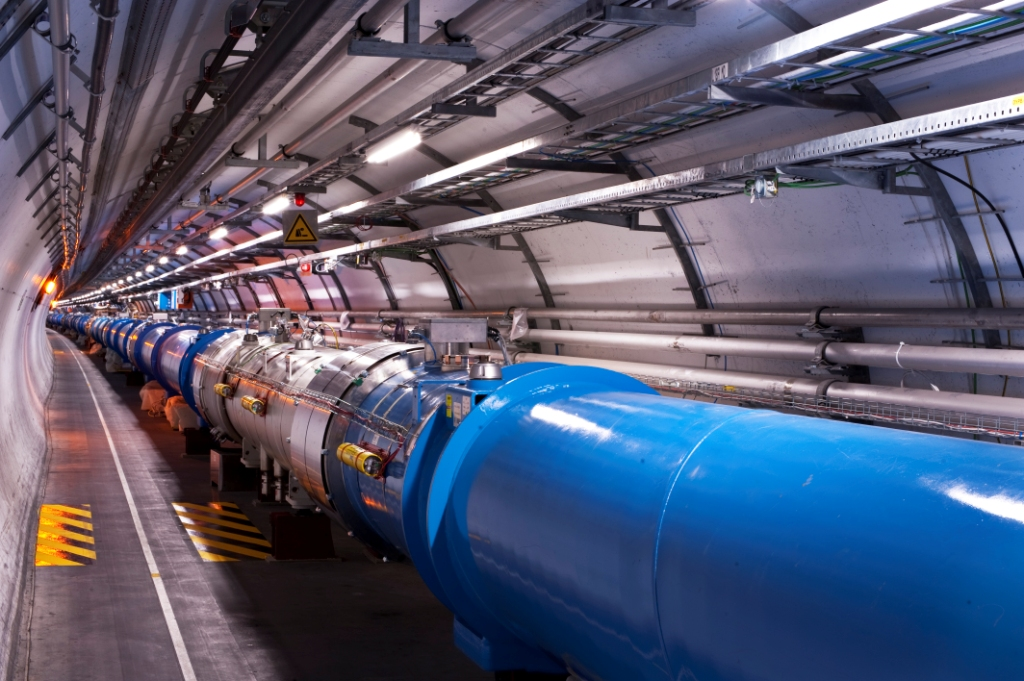
\includegraphics[width=200pt]{figures/theory/lhc_cern_compressed.jpg}
    %\end{figure}
  %\end{frame}
  %\begin{frame}{LWFA}{A plasma--based chraged particles accelerator}
  %Electrical breakdown is part of the design.

  %The power source is not microwave radiation, but either a laser beam or a charged particle beam.
  %\begin{figure}
    %%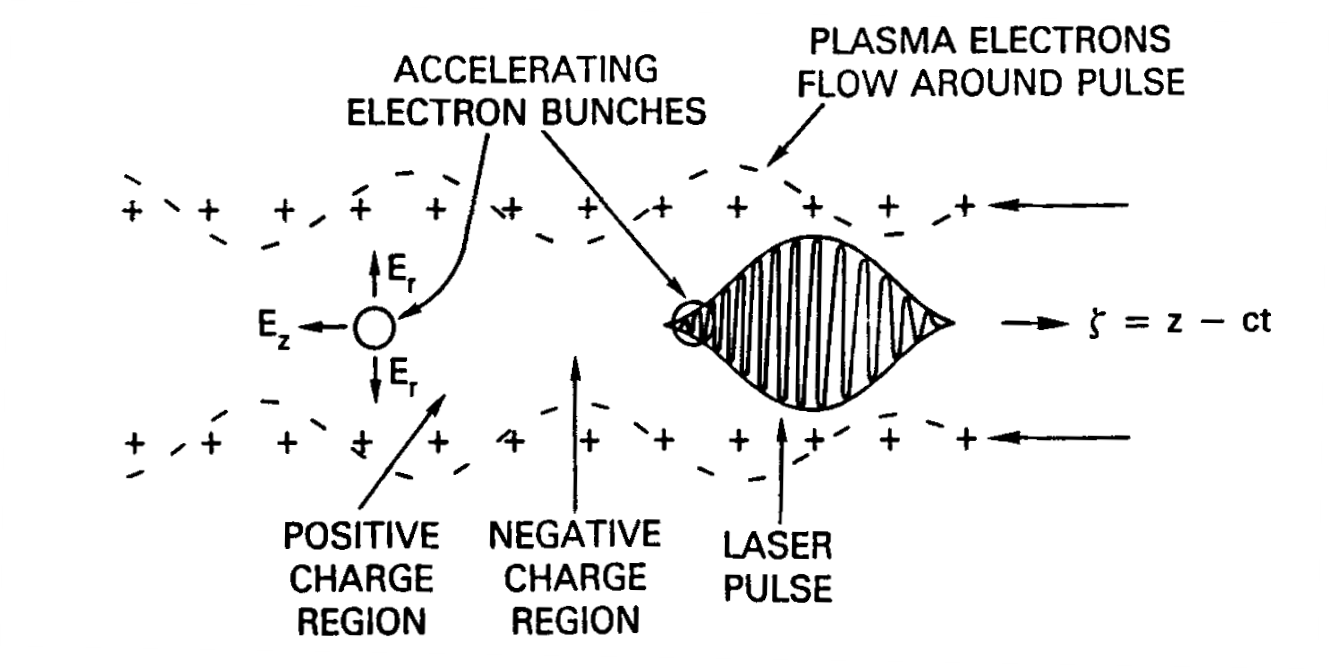
\includegraphics[width=300pt,height=150pt]{figures/theory/lwfa-schematic.tikz}
  %\end{figure}
  %\end{frame}
  %\begin{frame}{Wake waves}
    %\begin{columns}  
        %\column{0.5\textwidth}
          %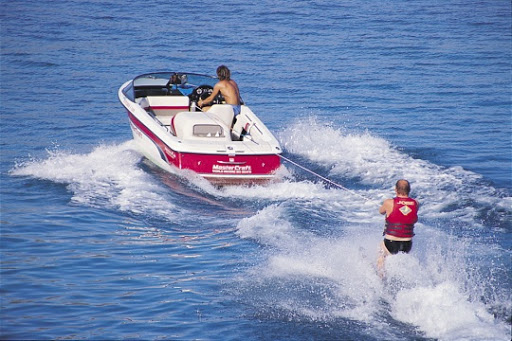
\includegraphics[width=\textwidth]{figures/theory/boat_ski.jpg}
        %\column{0.5\textwidth}
          %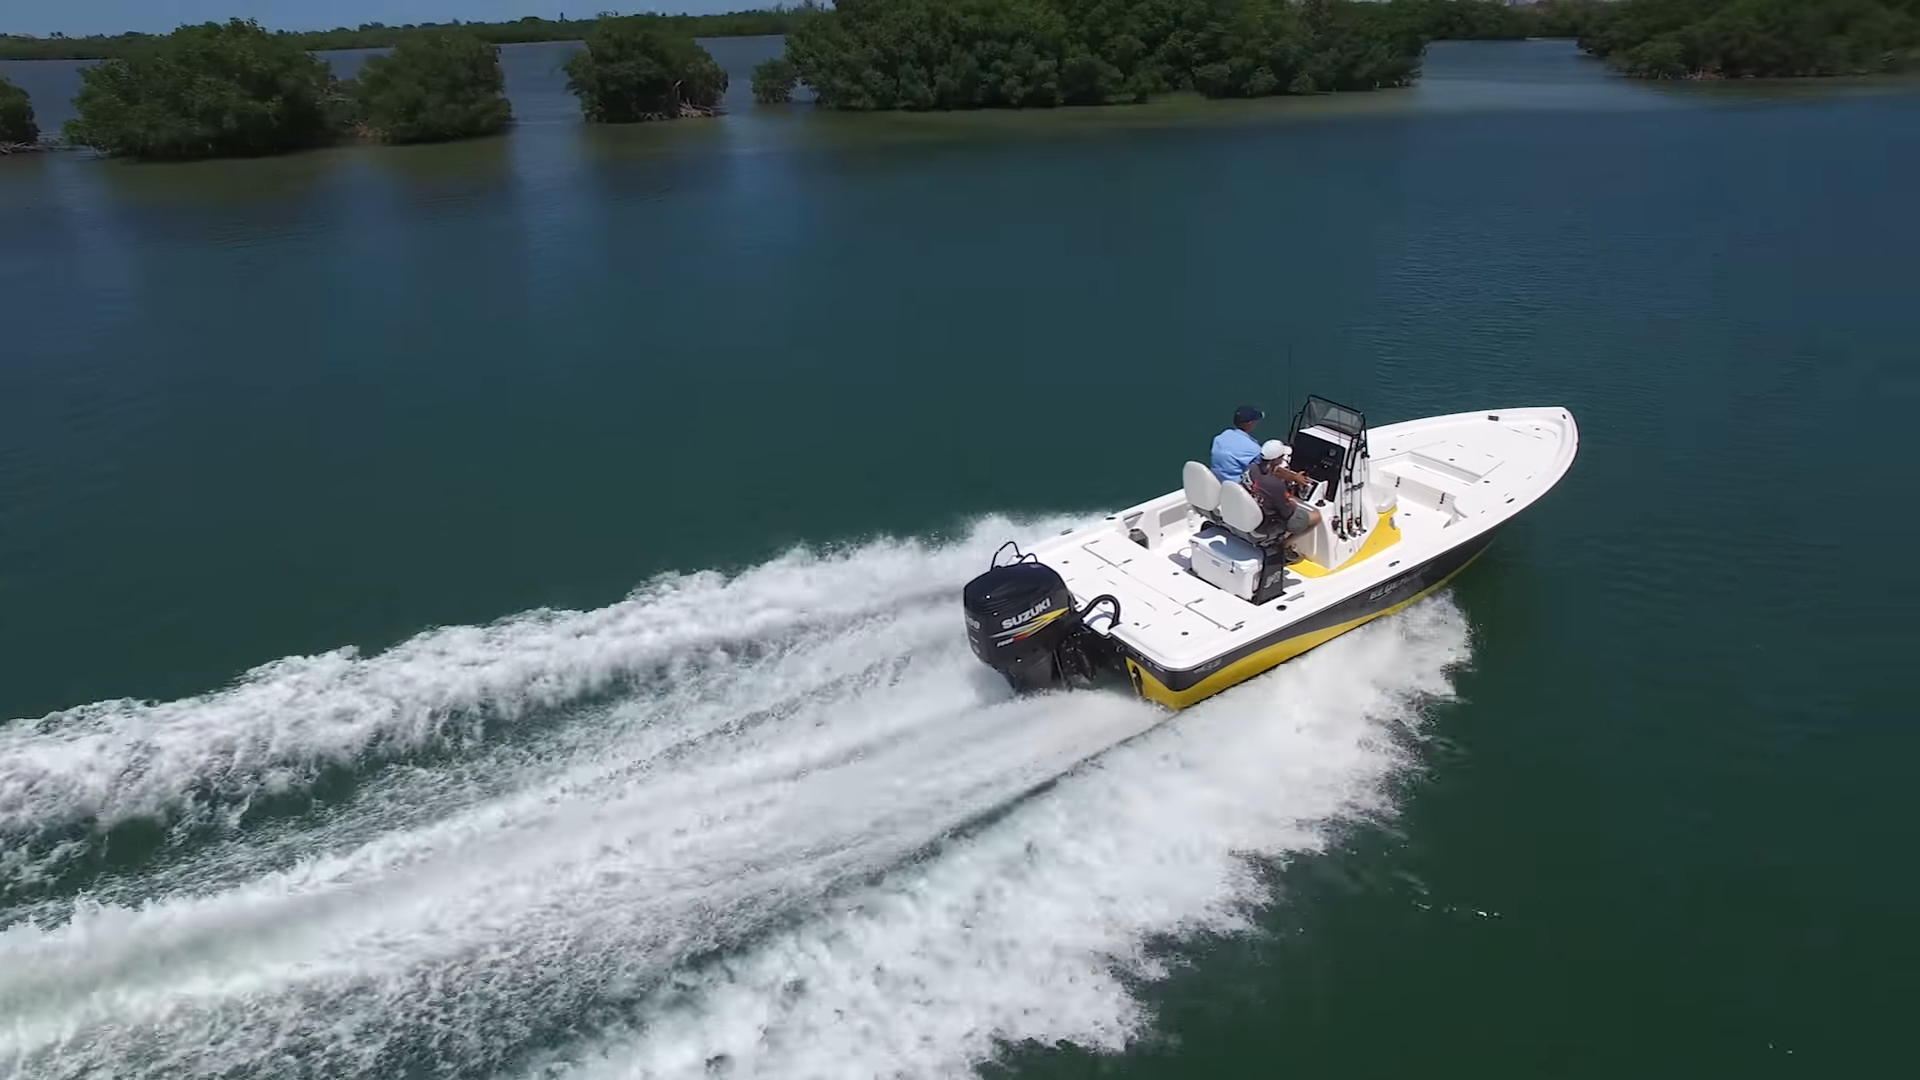
\includegraphics[width=\textwidth]{figures/theory/boat_wake.jpg}
    %\end{columns}
  %\end{frame}
  %%\begin{frame}{LWFA}{Limitations}
    %%\begin{columns}  
        %%\column<1,3>{0.5\textwidth}
    %%Laser defocusing
      %%\begin{figure}
          %%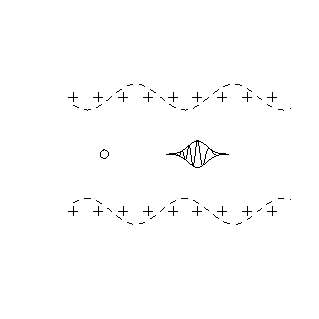
\includegraphics[width=\textwidth]{figures/theory/defocusing.tikz}
      %%\end{figure}
        %%\column<2,3>{0.5\textwidth}
      %%Electron dephasing
      %%\begin{figure}
          %%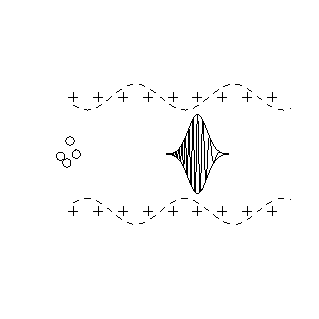
\includegraphics[width=\textwidth]{figures/theory/dephasing.tikz}
      %%\end{figure}
    %%\end{columns}
  %%\end{frame}
  %\begin{frame}{Beam divergence}
    %The divergence of a laser beam is usually neglected.

    %In LWFA, acceleration is achieved only when the laser beam is focused to $\sim$ tens of \si{\um} in diameter.
    %\begin{center}
      %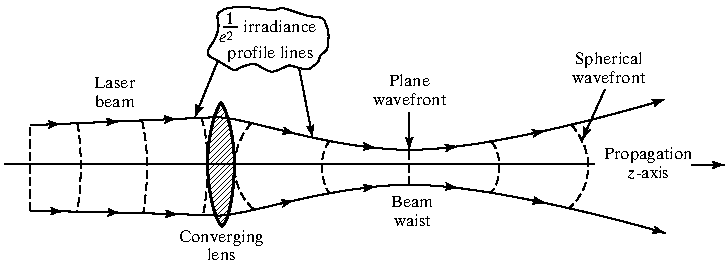
\includegraphics[width=\textwidth]{figures/theory/laser_lens_rayleigh.pdf}
    %\end{center}
    %Solution: Use a waveguide.
  %\end{frame}
  %\begin{frame}{Waveguide}{Basic concept}
  %\begin{figure}
     %%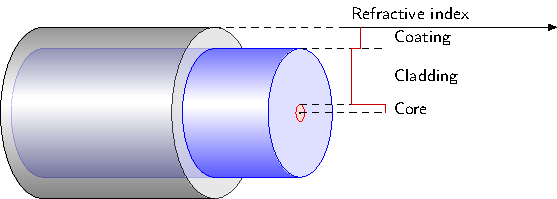
\includegraphics[width=0.8\textwidth]{figures/fiber.tikz}
   %\end{figure}
   %Light confined in core, cladding with a smaller refractive index.
  %\end{frame}
  %\begin{frame}{Construct a plasma waveguide}{Capillary Discharge Waveguide}
    %The plasma channel
    %\begin{itemize}
      %\item[\textbullet] forms dynamically,
      %\item[\textbullet] continuous radial decrease of $\tilde n$,
      %\item[\textbullet] results from the increase of plasma density
    %\end{itemize}
  %\end{frame}
  %\begin{frame}{Dephasing length}
    %To overcome the dephasing length limitation, a multi--stage accelerator, composed of multiple stages.
    %\begin{columns}
      %\column{0.5\textwidth}
      %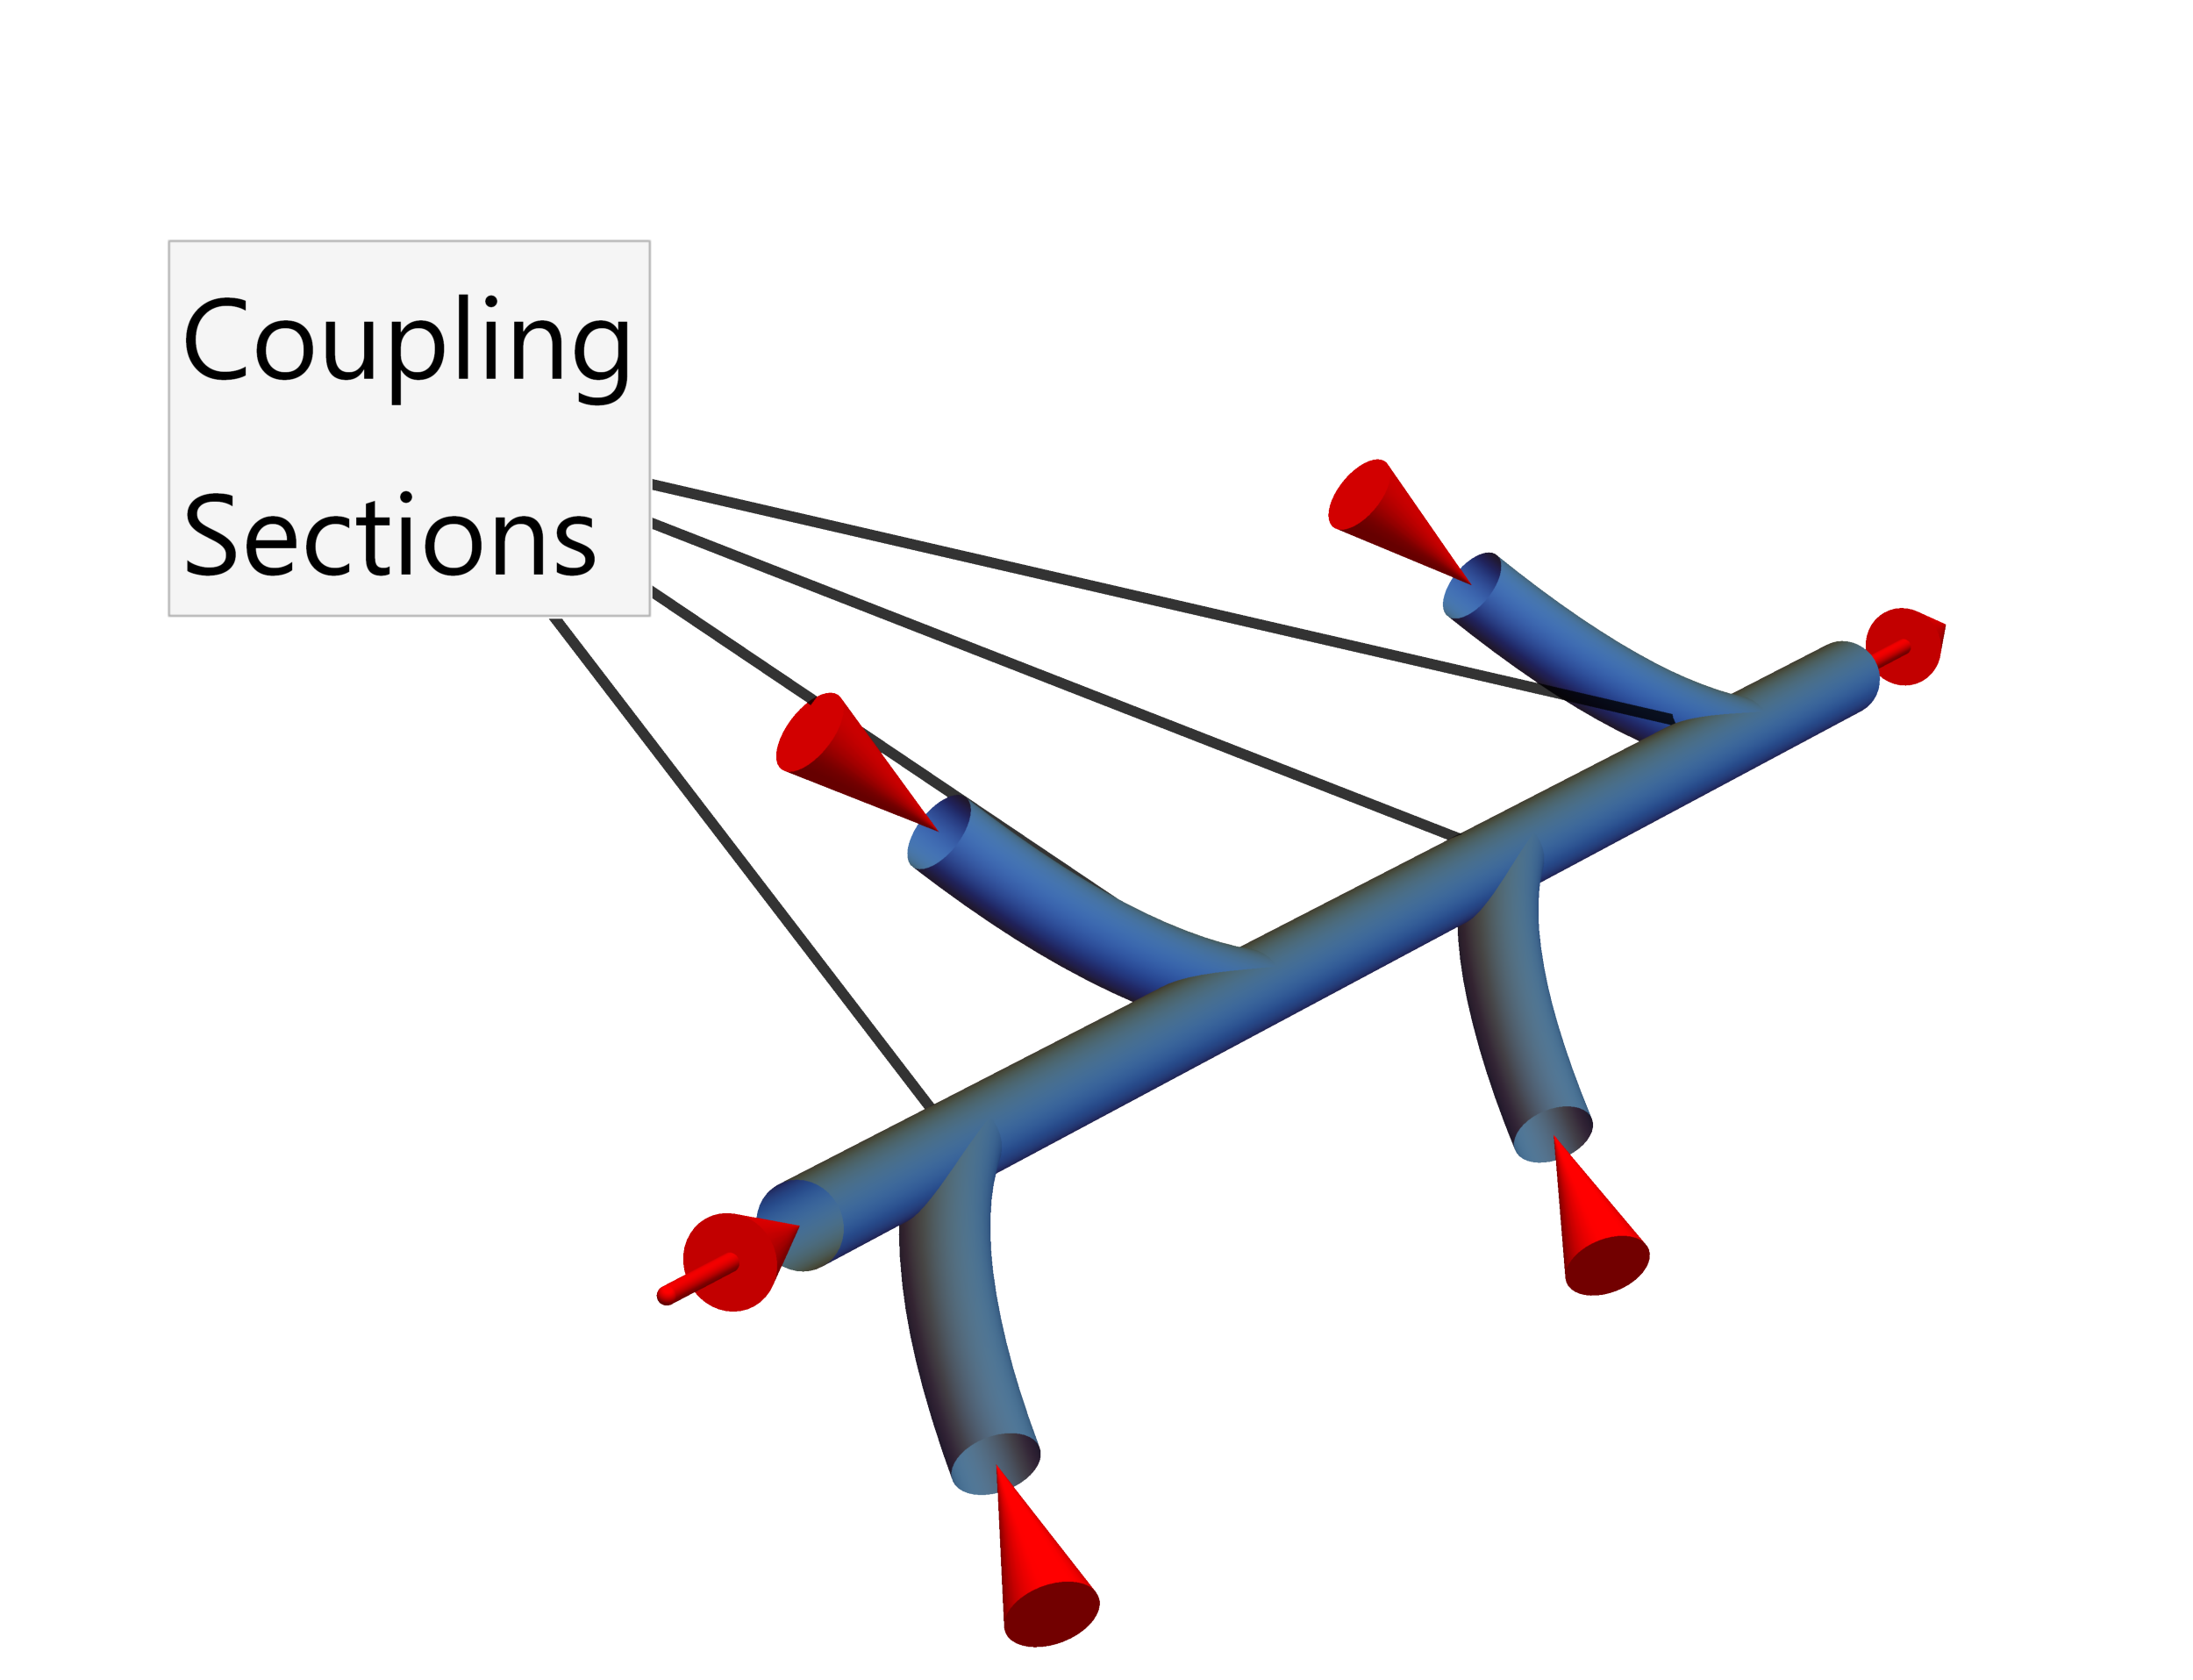
\includegraphics[width=\textwidth]{figures/coupling_scheme.pdf}
      %\column{0.5\textwidth}
      %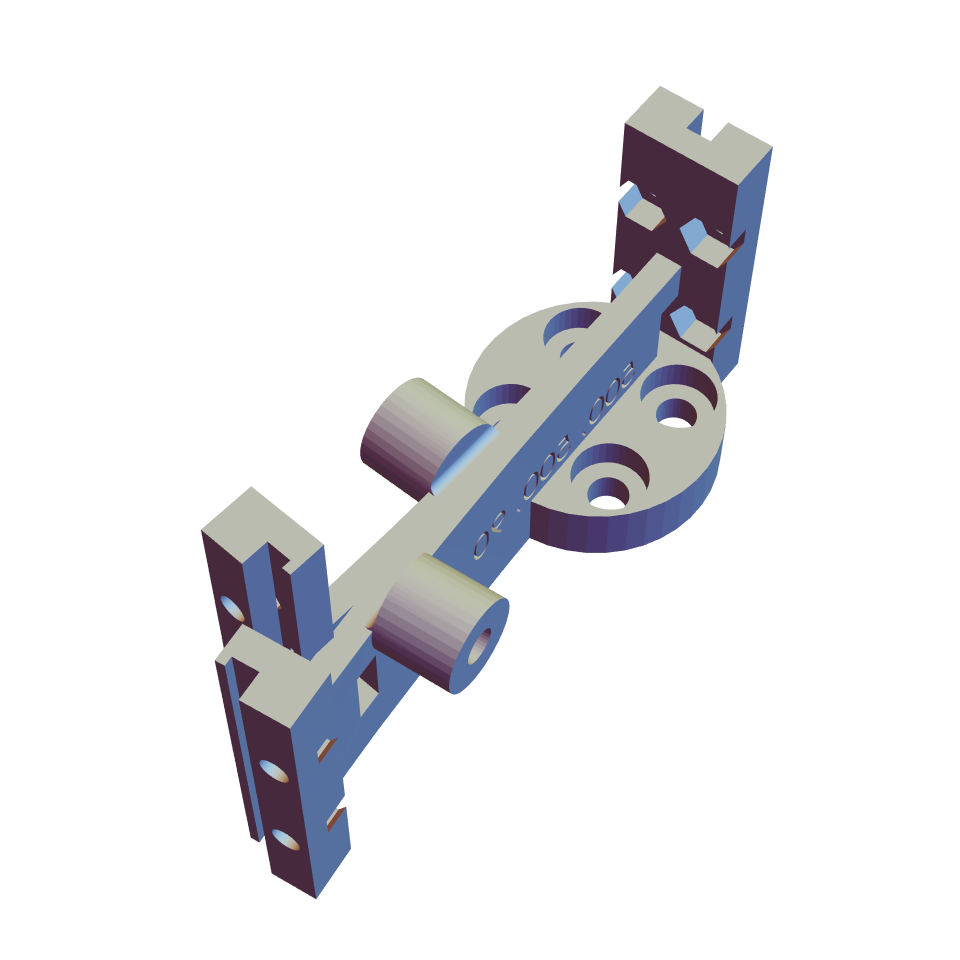
\includegraphics[width=\textwidth]{figures/theory/double_capillary_cad.png}
    %\end{columns}
  %\end{frame}
  %\subsection{Background to plasma}
  %\begin{frame}{Measures}
    %\begin{tabular}{l c r}
    %\onslide<1-> Debye length & $\lambda_D=\sqrt{\frac{\varepsilon_0 k_B T_e}{N_e e^2}}$ &  \\ 
    %\onslide<2-> Plasma Frequency & $ \omega_p=\sqrt{\frac{N_e e^2}{m_e \varepsilon_0}}\si[per-mode=fraction]{\radian\per\sec} $ &   \\
    %\onslide<3-> Plasma parameter & $ \Lambda=4\pi N_e \lambda_D ^3 $ &  \\
    %\end{tabular}
  %\end{frame}
  %\begin{frame}{}
      %\begin{table}[]
    %\begin{tabular}{l | c}
      %& T$\sim$\SI{1}{\electronvolt},$N_e\sim\SI{e17}{\per\cubic\cm}$ \\ \hline 
      %$\lambda_D$     & \SI{33}{\nm}     \\
      %$\omega_p$      & $\SI[per-mode=fraction]{e13}{\radian\per\sec}$   \\
      %$\Lambda$ & 40
    %\end{tabular}
      %\end{table}
  %Plasmas in LWFA environments require
    %\begin{enumerate}
      %\item[\textbullet] overall quasi-neutrality
      %\item[\textbullet] hot plasma, yet underdense --- $\Lambda \gg 1$
    %\end{enumerate}
  %\end{frame}
%\subsection{Plasma spectroscopy}
%\begin{frame}{Plasma spectroscopy}{Electron density measurement}
%Study of the emitted spectra gives information on the plasma.
%\vskip 2em
%\begin{tabular}{c c}
 %%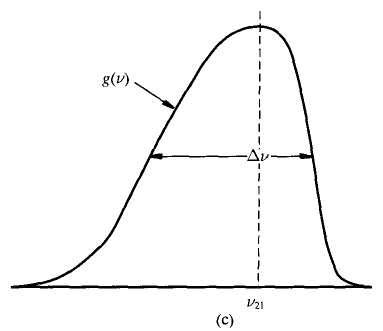
\includegraphics[width=0.5\textwidth,height=0.3\textwidth]{figures/theory/lineshape.tikz} 
 %&
 %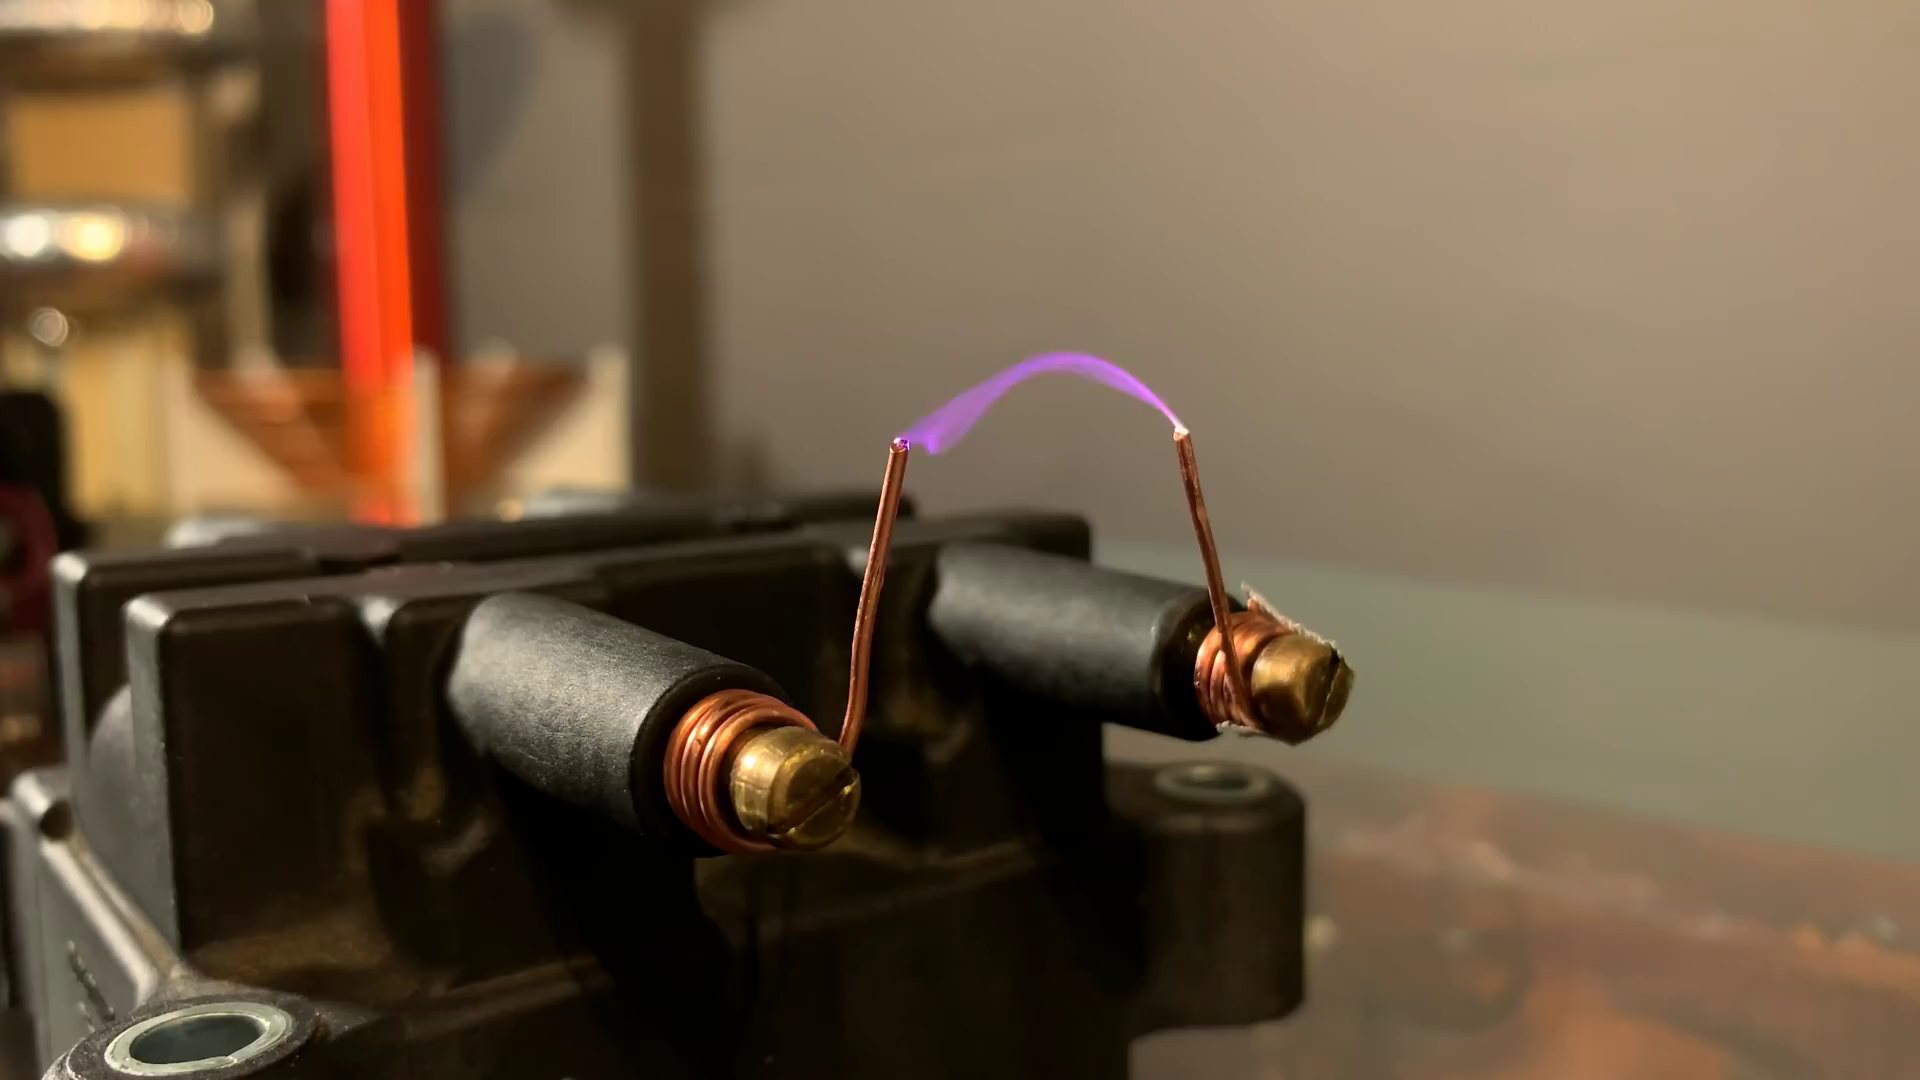
\includegraphics[width=0.5\textwidth]{figures/theory/purple_plasma.png}
%\end{tabular}
%\begin{center}
  %\vskip 1em
%Plasma diagnostic under a theoretical model --- the LTE model.
%\end{center}
%\end{frame}
%\begin{frame}{Optical Depth}{Optically thin plasma}
  %Optical depth $\tau$ \small{(dimensionless)} --- a measure of the opacity of the medium:
  %\begin{equation*}
    %\tau=-\kappa z
  %\end{equation*}
  %$\kappa$ --- the linear absorption coefficient (\si{\per\cm}).

  %$I_\text{out}$ and $I_\text{in}$ are related by
  %\begin{equation*}
    %I_\text{out} = I_\text{in}\mathrm{e}^{-\kappa z} %\tag{(Simplest)radiative transfer equation}
  %\end{equation*}
%\begin{columns}
  %\column{0.4\textwidth}
      %%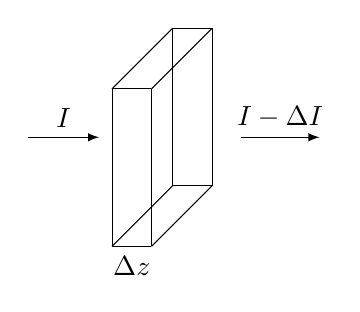
\begin{tikzpicture}
\draw(-0.25,1,1) -- (0.25,1,1);
\draw(-0.25,1,1) -- (-0.25,1,-1);
\draw(-0.25,1,1) -- (-0.25,-1,1);
\draw(0.25,1,1) -- (0.25,1,-1);
\draw(0.25,1,1) -- (0.25,-1,1);
\draw(0.25,1,-1) -- (-0.25,1,-1);
\draw(0.25,1,-1) -- (0.25,-1,-1);
\draw(-0.25,1,-1) -- (-0.25,-1,-1);
\draw(-0.25,-1,1) -- node [midway, below] {$\Delta z$} (0.25,-1,1);
\draw(0.25,-1,-1) -- (0.25,-1,1);
\draw(0.25,-1,-1) -- (-0.25,-1,-1);
\draw(-0.25,-1,-1) -- (-0.25,-1,1);
\draw[-latex] (-1.7,0,0) -- node [midway, above] {$I$} (-0.8,0,0);
\draw[-latex] (1,0,0) --  node [midway, above] {$I-\Delta I$} (2,0,0) ;


\end{tikzpicture}

    %\column{0.6\textwidth}
  %\begin{center}
  %\begin{tabular}{ c c c }
    %$\tau<1$ & $\longrightarrow$ & optically thin medium\\ 
    %$\tau>1$ & $\longrightarrow$ & optically thick medium
  %\end{tabular}
  %\end{center}
%\end{columns}
%\end{frame}
\begin{frame}{Local Thermodynamic Equilibrium (LTE) Model}
  Particle collision processes dominate over radiative processes.
  \begin{figure}
    \includegraphics[width=0.7\textwidth]{figures/theory/processes.tikz}
  \end{figure}
  %Population densities of the electrons is determined by particle collision processes (and not by radiative process).

  % Thorne figure 13.6. Hutchinson page 224 lists the electron processes.

  Instantaneous respnse to any change in plasma conditions (detailed balance)
  % The electron distribution responds instantaneously to any change in plasma conditions (detailed balance).
\end{frame}

%\begin{frame}{Stark Broadening}
  %Plasma is a charged medium.

  %Electric micro--fields perturb the atomic energy levels.

  %Averaging over different neighbours converts the Stark splitting to Stark broadening.
  %\begin{figure}
  %%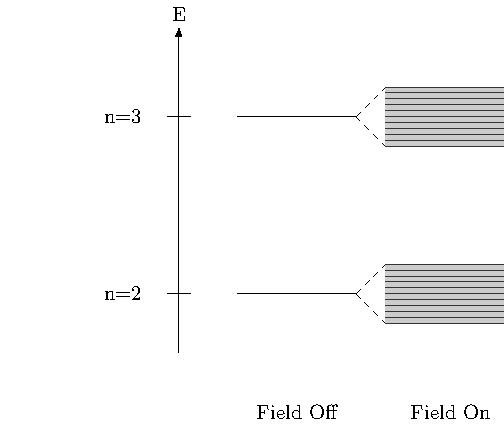
\includegraphics[width=0.5\textwidth]{figures/theory/starkBroadening.tikz}
  %\end{figure}
%\end{frame}
%\begin{frame}{Stark Broadening}
  %Lorentzian line shape --- $I\left( \lambda \right)=\dfrac{A^2}{4\left( \left(\lambda-\lambda_0\right)^2+\Delta \lambda_{1/2}^2\right)}$
  %%\begin{equation*}
    %%I\left( \lambda \right)=\frac{A^2}{4\left( \left(\lambda-\lambda_0\right)^2+\Delta \lambda_{1/2}^2\right)}
  %%\end{equation*}
  %\vskip 1.5em
  %\begin{columns}
    %\column{0.4\textwidth}
    %\begin{figure}
      %%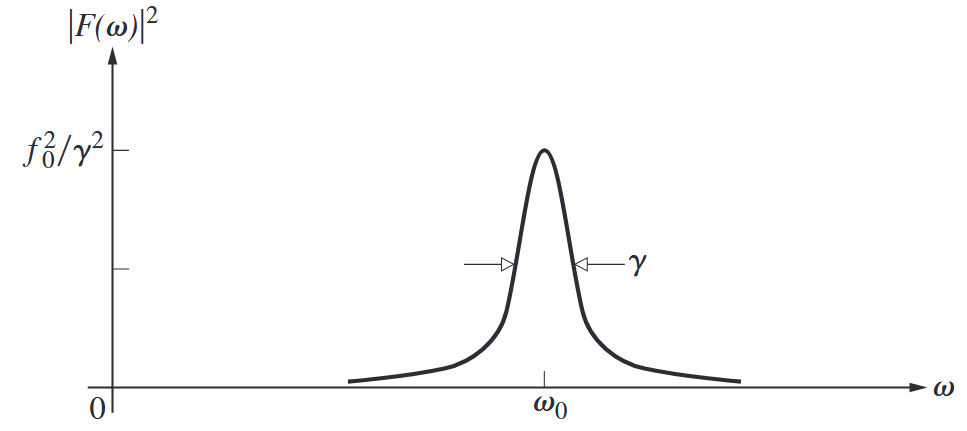
\includegraphics[width=\textwidth,height=0.7\textwidth]{figures/lorentzian_lineshape.tikz}
    %\end{figure}
    %\column{0.6\textwidth}
    %Relation between $N_e$ and $\Delta \lambda_{1/2}$ is tabulated: $$N_e=\left( \frac{\Delta\lambda_{1/2}}{\gamma\left(n_e,T_e\right)}\right)^{3/2}.$$
    %\\
    %Weak dependence on temperature, in our experiment: $$N_e\left[\SI{e18}{\per\cubic\cm}\right]=\left( \frac{\Delta\lambda_{1/2}\left[\si{\nm}\right]}{5.4}\right)^{3/2}.$$
  %\end{columns}
%\end{frame}
%\subsection{Preformed Plasma channel}
%\begin{frame}{Parabolic density profile}
  %Ideally, the radial density profile (RDP) is parabolic:
    %\begin{equation*}
    %N_e(r)=N_e(0)+\Delta N_e\left( \frac{r}{r_\text{ch}}\right)^2
  %\end{equation*}
  %\begin{columns}
   %\column{0.5\textwidth} 
    %%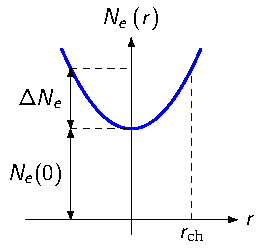
\includegraphics[height=0.9\textwidth]{figures/theory/rdp.tikz}
   %\column{0.5\textwidth} 
    %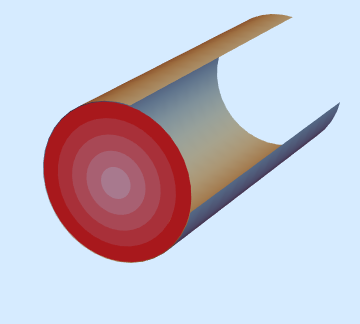
\includegraphics[width=\textwidth]{figures/theory/why channel forms.png}
  %\end{columns}
%\end{frame}
%\begin{frame}{Creating a plasma channel}
    %\begin{itemize}
      %\item Ablated capillary
      %\item Gas--filled capillary
    %\end{itemize}
    %\begin{tabular}{cc}
    %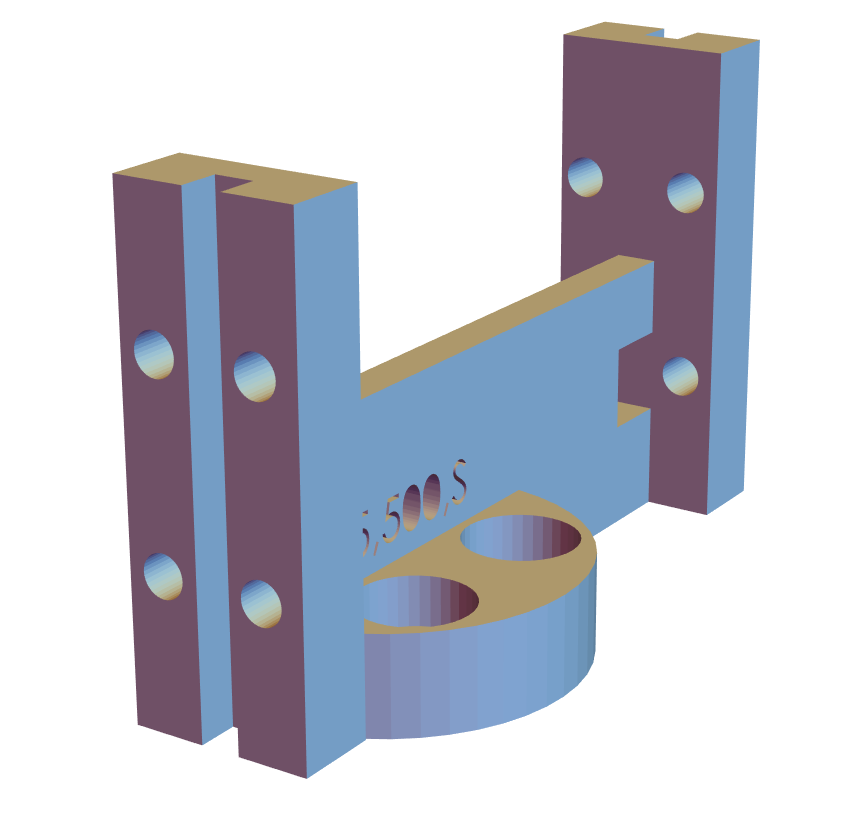
\includegraphics[width=0.5\textwidth]{figures/theory/ablated.png} & 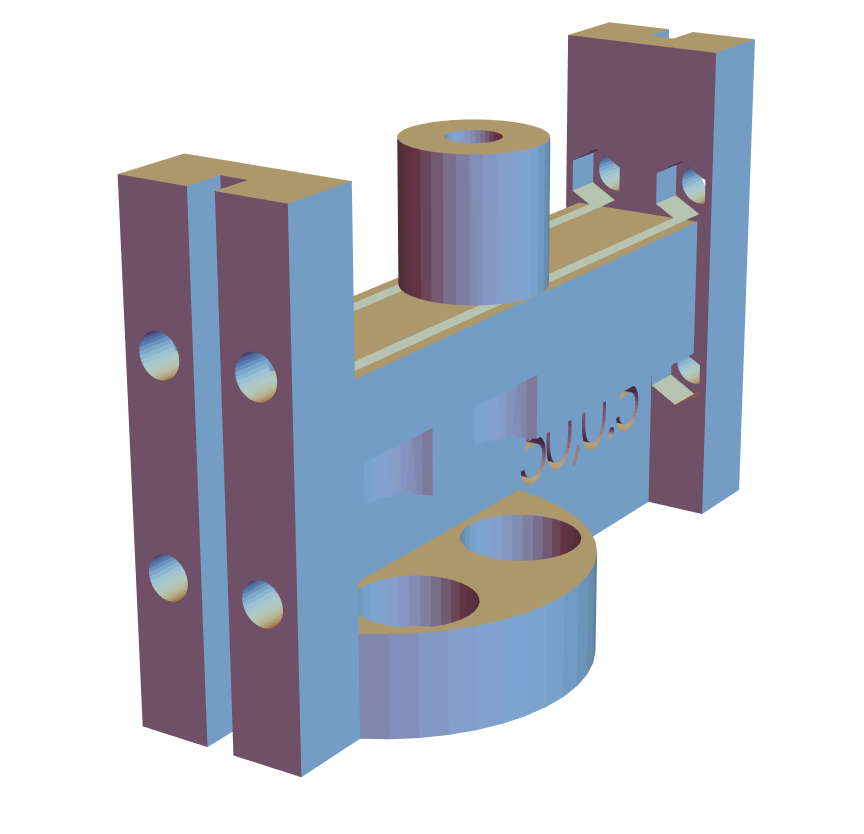
\includegraphics[width=0.5\textwidth]{figures/theory/gasfilled.png}
    %\end{tabular}
%\end{frame}
%\section{Thesis Goals}
%\begin{frame}{Thesis Goals}
  %\begin{enumerate}
    %\item Study of discharge evolution, low jitter of discharge ignition.
    %\item Demonstration of optical guiding.
    %\item Spectroscopy analysis, utilizing Stark broadening.
    %\item Development of multi stage capillary --- fish bone approach.
  %\end{enumerate}
%\end{frame}
%\section{Experiment Scheme}
%\begin{frame}{Experiment Scheme}
  %\begin{figure}
    %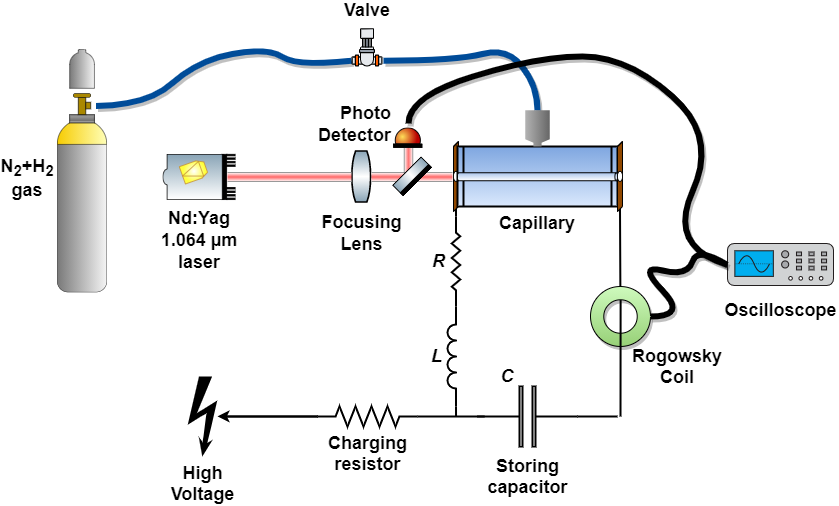
\includegraphics[width=\textwidth]{figures/methods/Laser-based ignition scheme.png}
  %\end{figure}
  %Capillary inside a vacuum chamber, maintained at \SI{e-4}{\torr}
%\end{frame}
%\begin{frame}{Experiment Scheme}{continued}
  %\begin{figure}
    %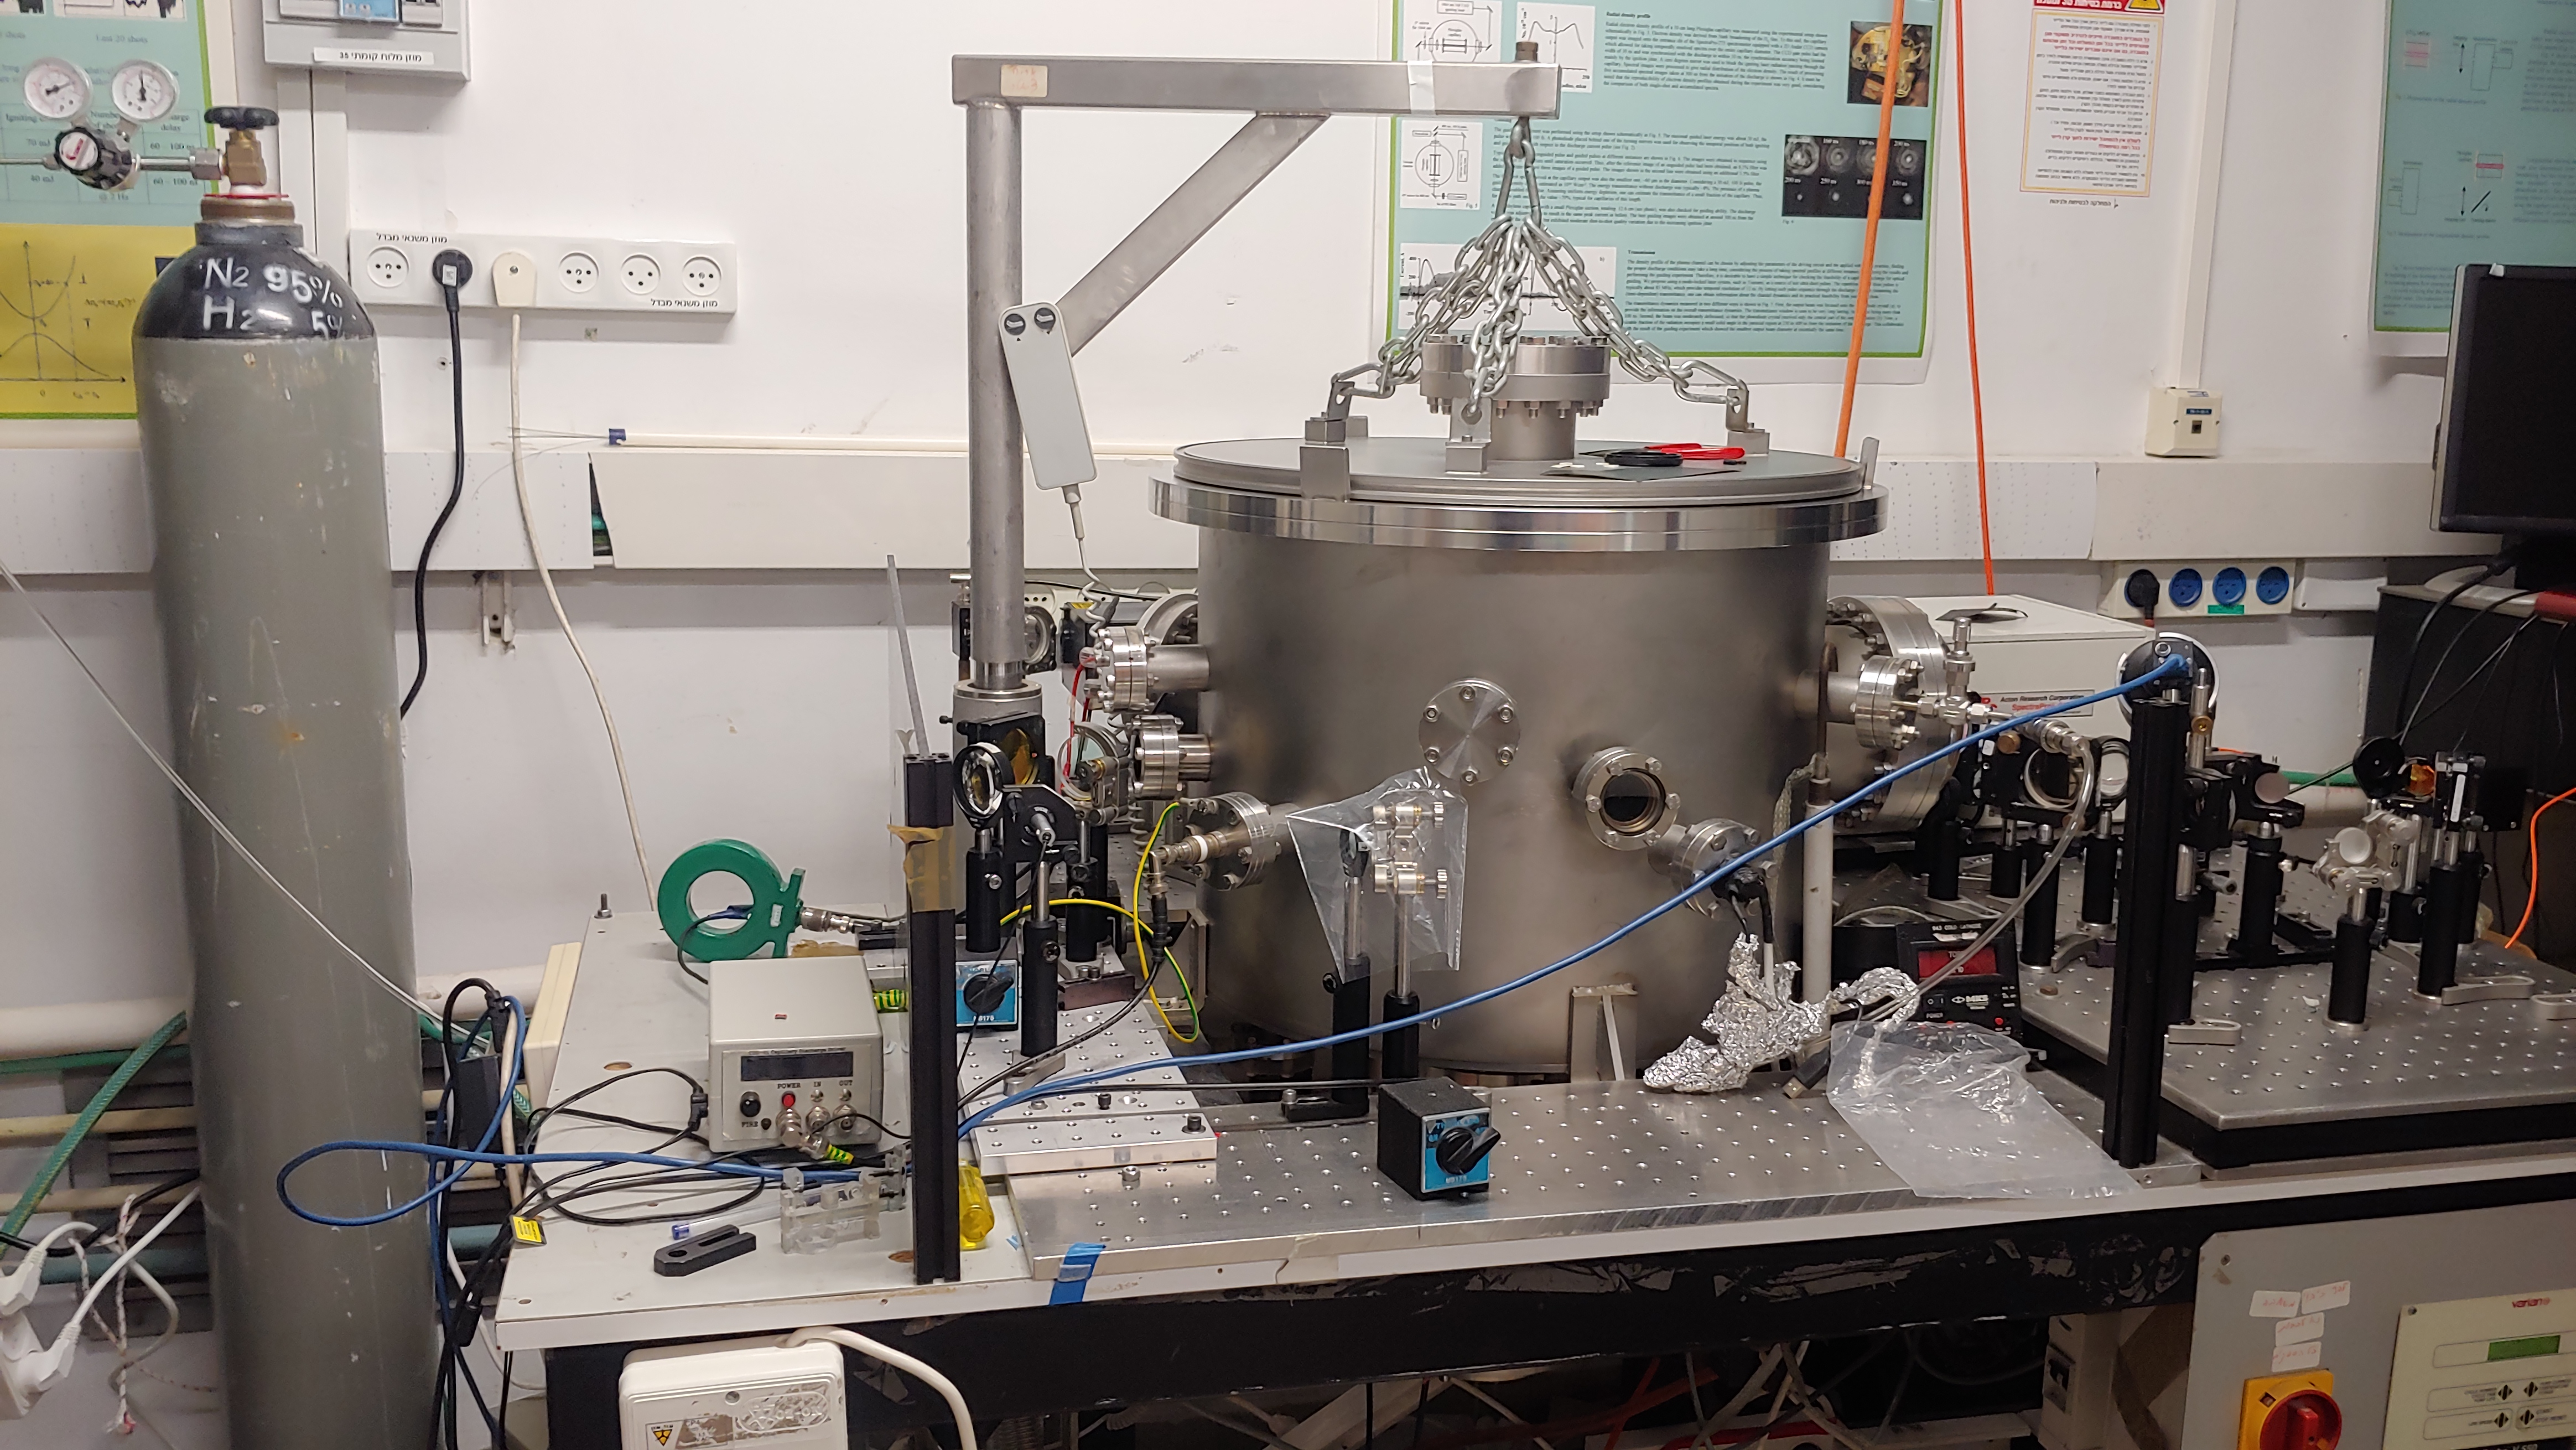
\includegraphics[width=\textwidth]{figures/methods/system_picture.jpg}
  %\end{figure}
%\end{frame}
%\section{Experimental Results}
%\subsection{Low Jitter}
%\begin{frame}{Experimental Results}{Low Jitter}
  %A typical plasma discharge. Damped oscillatory current profile.
  %\begin{figure}
    %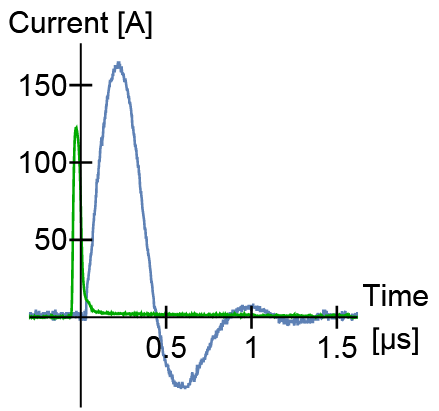
\includegraphics[width=0.5\textwidth]{figures/results/typical.png}
  %\end{figure}
  %Requirement for a ready--to--use guiding media --- low jitter.
%\end{frame}
%\begin{frame}{Experimental Results}{Low Jitter}
  %12 cosecutive capillary discharges. Demonstrating low ignition jitter.
  %\begin{figure}
    %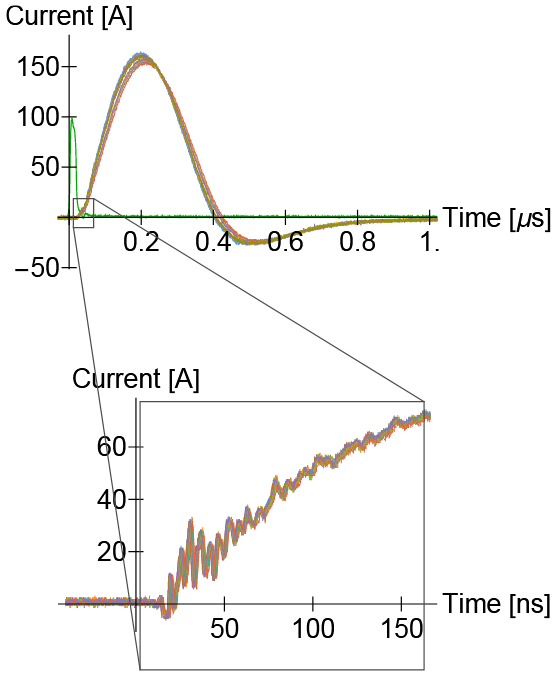
\includegraphics[width=0.4\textwidth]{figures/results/low_jitter.png}
  %\end{figure}
  %$$\tau_\text{jitter}\approx 1\pm 0.36 \si{\ns}$$
%\end{frame}
%\begin{frame}{Experimental Results}{Low Jitter}
  %Without the igniting laser pulse - much less stable regime.
  %\begin{figure}
    %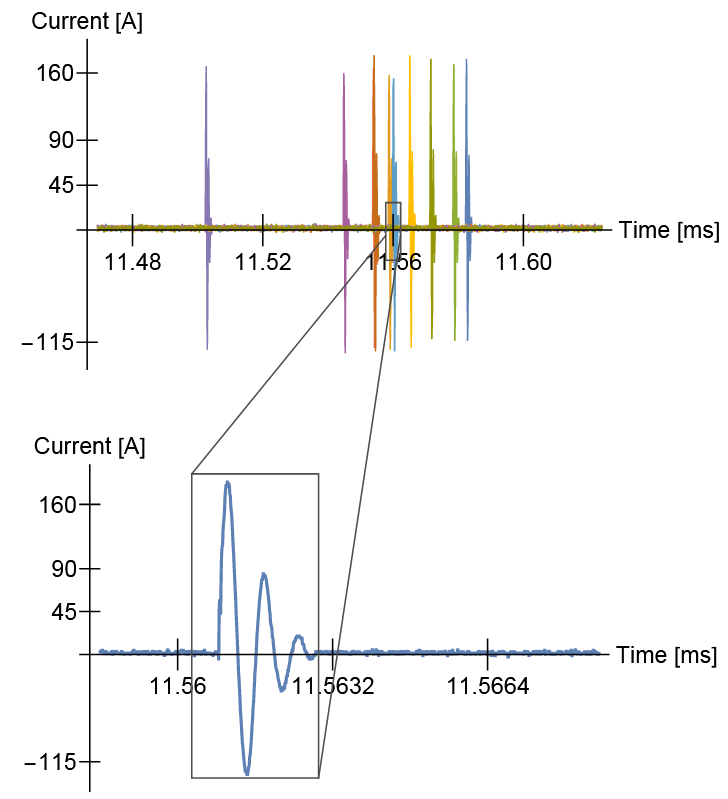
\includegraphics[width=0.4\textwidth]{figures/results/high_jitter.png}
  %\end{figure}
  %$$\text{jitter}\approx \SI{80}{\us}$$
%\end{frame}
%\subsection{Optical Guiding}
  %\begin{frame}{optical guiding}{System setup}
    %System setup as before, but now adding an oscillator laser.
    %\begin{figure}
     %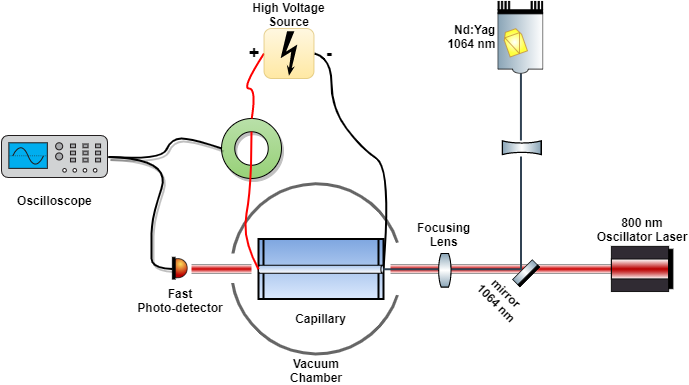
\includegraphics[width=\textwidth]{figures/results/oscillator/oscillator_system_setup.png} 
    %\end{figure}
    %Beam aligned throught the capillary, to a fast photo--diode.
  %\end{frame}
  %\begin{frame}{Oscillator laser}{Temporal profile}
    %Oscillator laser, \SI{800}{\nm}, pulses at a \SI{84}{\MHz} rate.
    %\begin{figure}
      %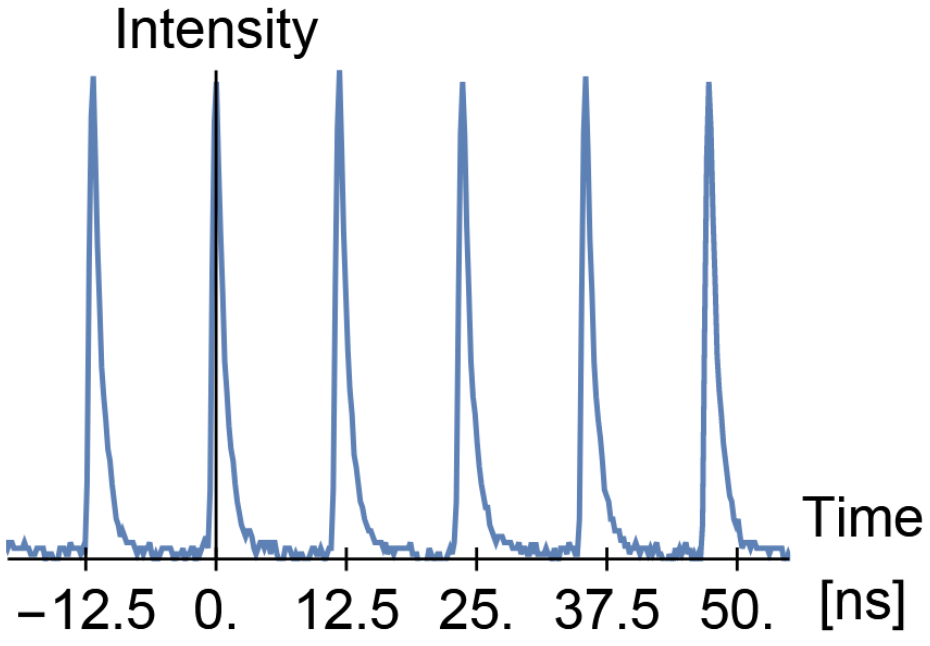
\includegraphics[width=0.4\textwidth]{figures/results/oscillator/single.PNG}
    %\end{figure}
  %\end{frame}
  %\begin{frame}{Optical Guiding}
    %Upon plasma discharge, we look for an increase in the detected amplitude --- optical guiding.
    %\begin{equation*}
      %\text{transmission ratio} = \frac{A_{t<0}}{A_\text{max}}
    %\end{equation*}
    %\begin{figure}
      %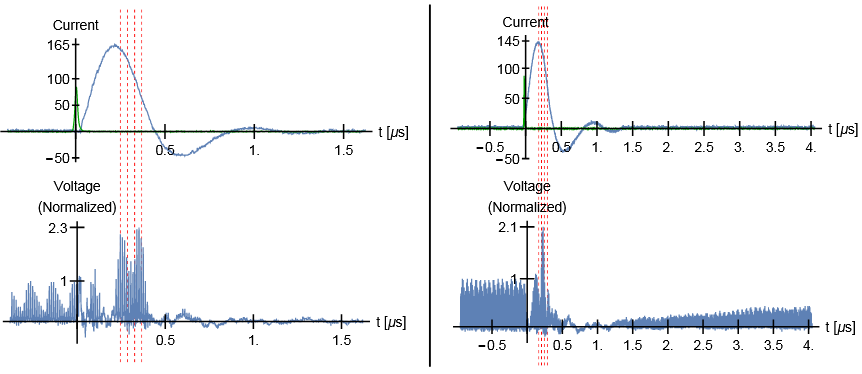
\includegraphics[width=\textwidth]{figures/results/oscillator/results01.PNG}
    %\end{figure}
  %\end{frame}
  %\begin{frame}
    %Another frame witht results02.png
  %\end{frame}
  %\begin{frame}{Optical guiding}{Explanation}
    %A plasma lens forms, the radiation is focused and trapped by the plasma.
    %\begin{figure}
      %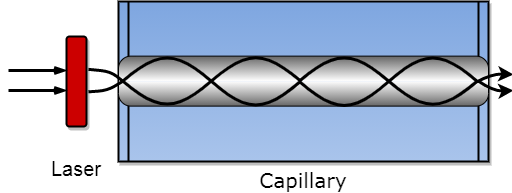
\includegraphics[width=0.3\textwidth]{figures/results/oscillator/chen4_31.png}
    %\end{figure}
    %Note: The radiation is blocked in the later stage of the discharge, until the plasma is diffused.
    %\begin{figure}
      %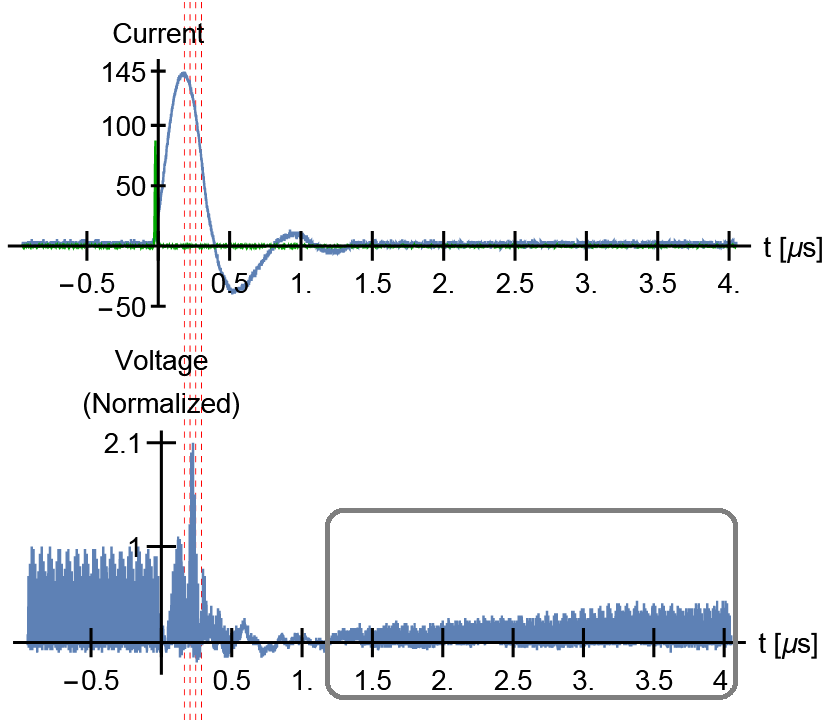
\includegraphics[width=0.4\textwidth]{figures/results/oscillator/not_opaque.PNG}
    %\end{figure}
  %\end{frame}
  %\begin{frame}{Duration of the plasma channel}
    %Correlation between applied voltage and the transmission ratio:
    %\begin{figure}
      %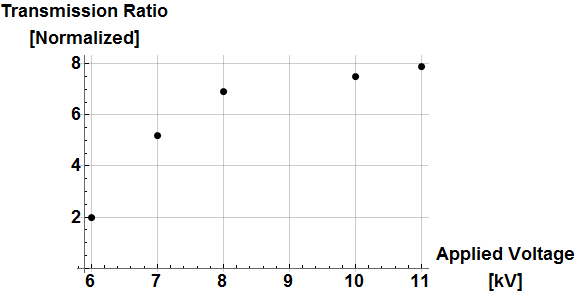
\includegraphics[width=0.4\textwidth]{figures/results/oscillator/voltage vs guiding.png}
    %\end{figure}
    %Duration of the plasma channel:
    %\begin{equation*}
      %\Delta t_\text{channel}=50 -100\ \si{\ns}.
    %\end{equation*}
  %\end{frame}
%\subsection{Spectroscopy measurement}
%\begin{frame}{Spectroscopy measurements}
  %\begin{itemize}
    %\item Quantitative estimation of the plasma channel depth and the plasma density
    %\item Both radial and longitudinal density profile
    %\item Method: A spectrometer and a fast camera
  %\end{itemize}
  %\begin{figure}
    %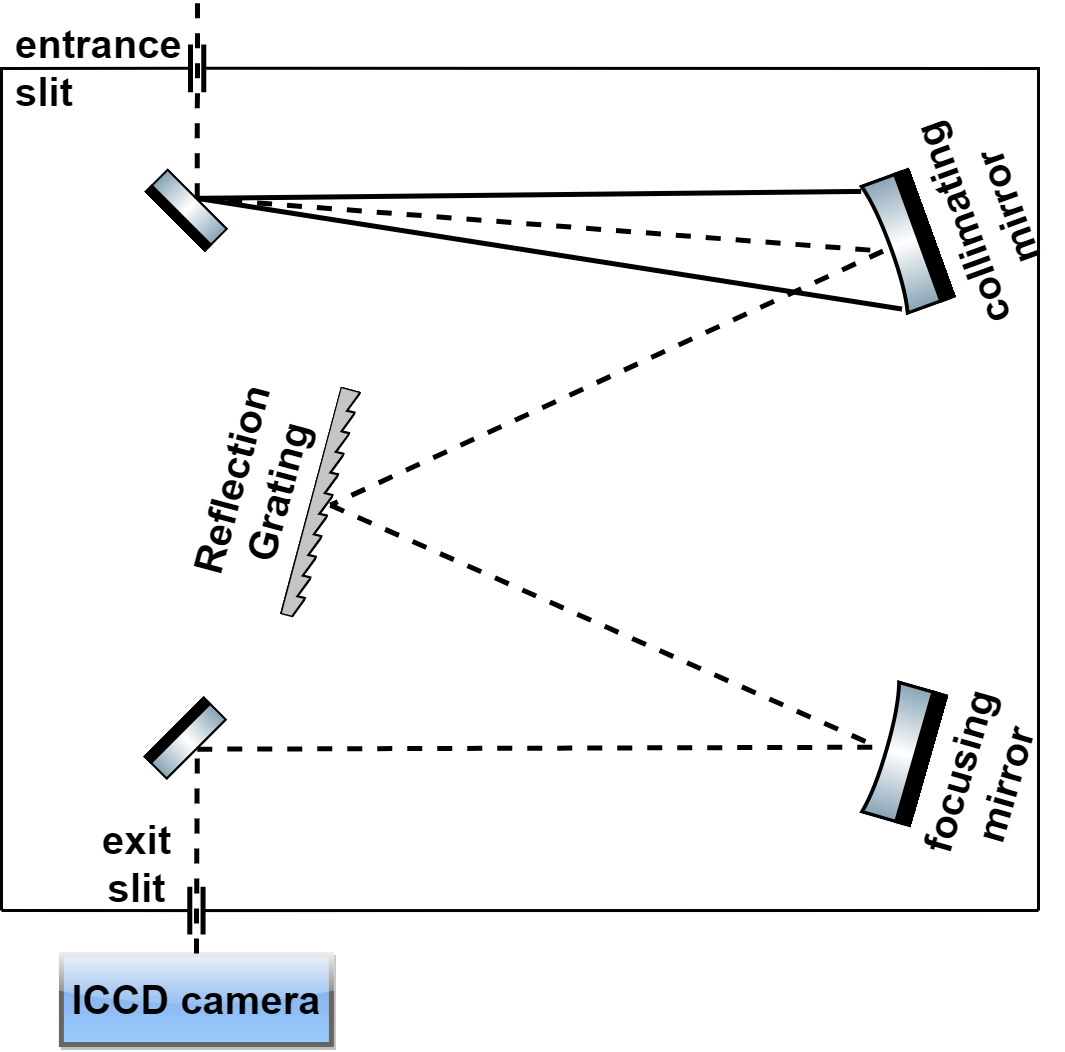
\includegraphics[height=140pt]{figures/results/spectro/spectrometer.png}
  %\end{figure}
%\end{frame}
%\begin{frame}{Radial density profile}
  %\begin{figure}
    %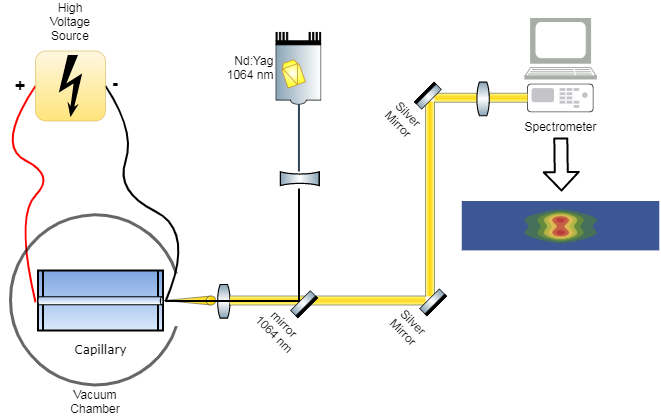
\includegraphics[width=0.8\textwidth]{figures/results/spectro/radial_system.png}
  %\end{figure}
%Imaging system --- $\times 5$ magnification.

%CCD camera $\SI{40}{\ns}$ gate--on time. 

%Width of the spectrometer slit --- \SI{150}{\um}.
%\end{frame}
%\begin{frame}{Spectroscopy Analysis}
  %\begin{figure}
    %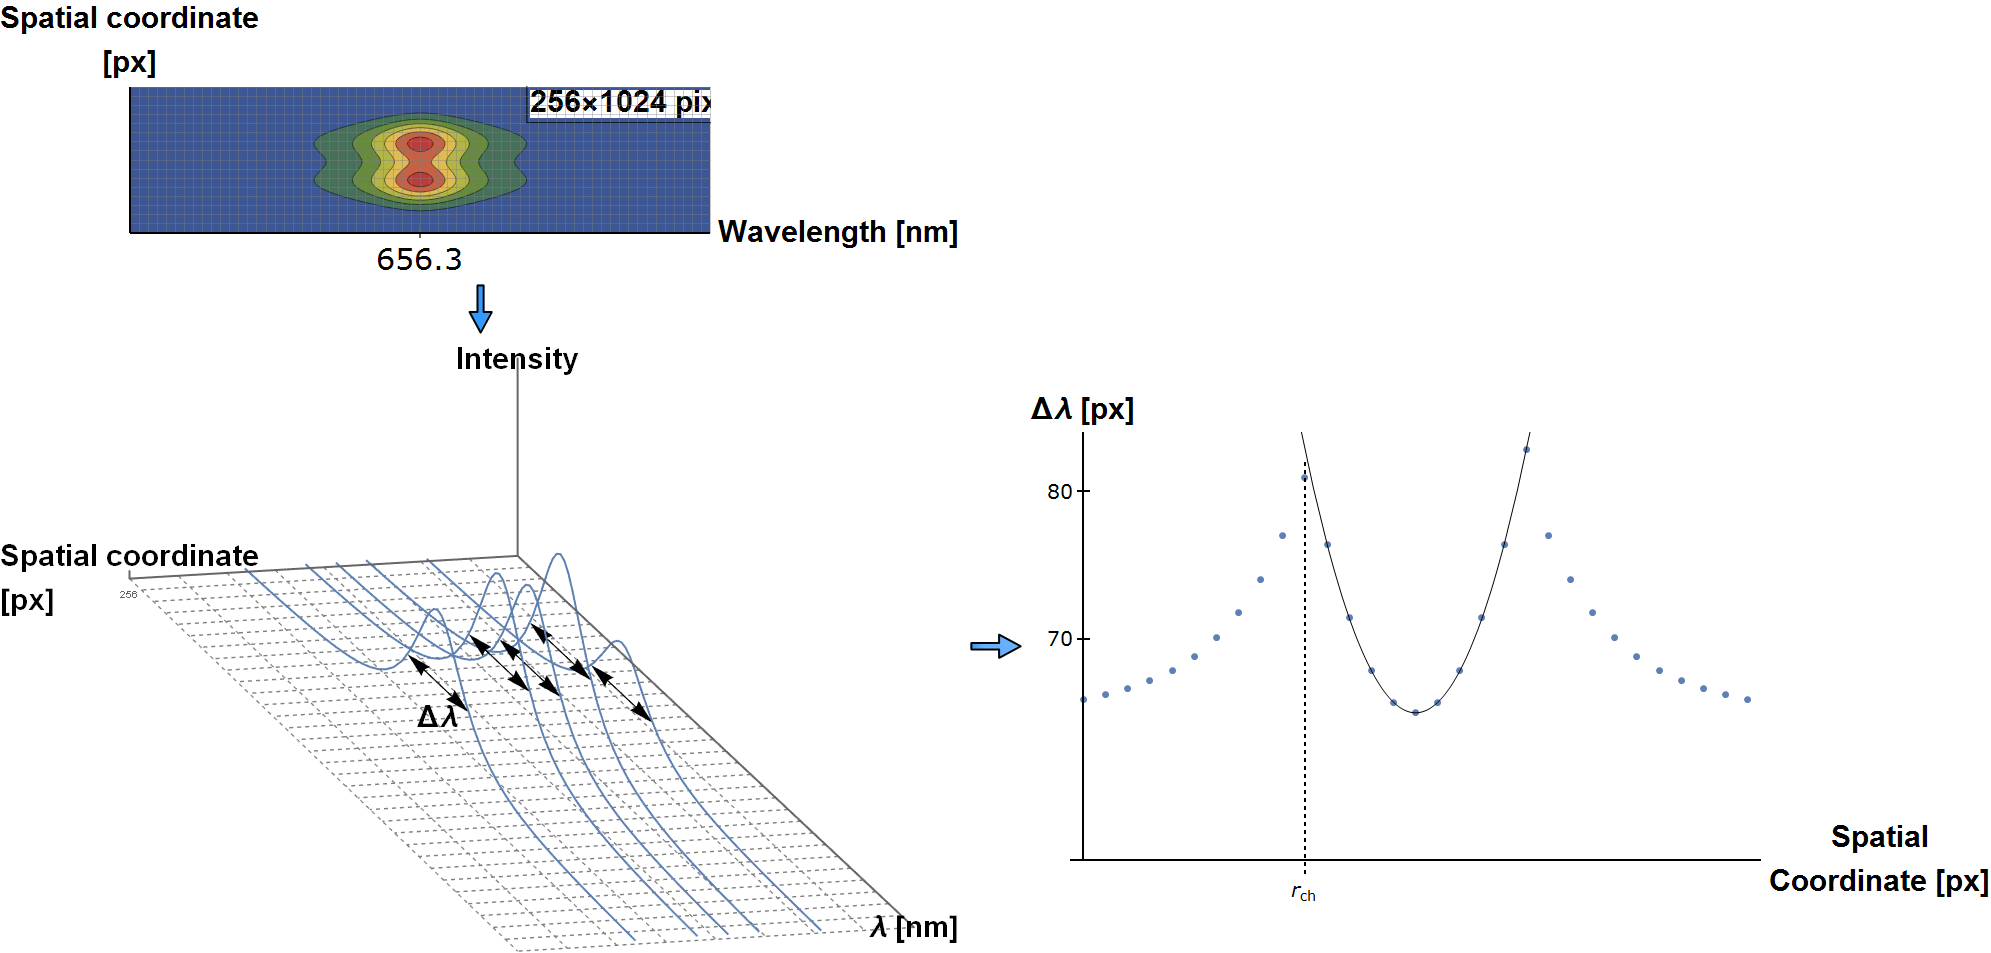
\includegraphics[width=0.8\textwidth]{figures/results/spectro/spectra_analysis.png}
  %\end{figure}
  %pixel size = $\SI{26}{\um} \times \SI{26}{\um}$
%\end{frame}
%\begin{frame}{Spectroscopy Analysis}{cont.}
    %Fit a Lorentzian to each row of the data.
    %\begin{figure}
      %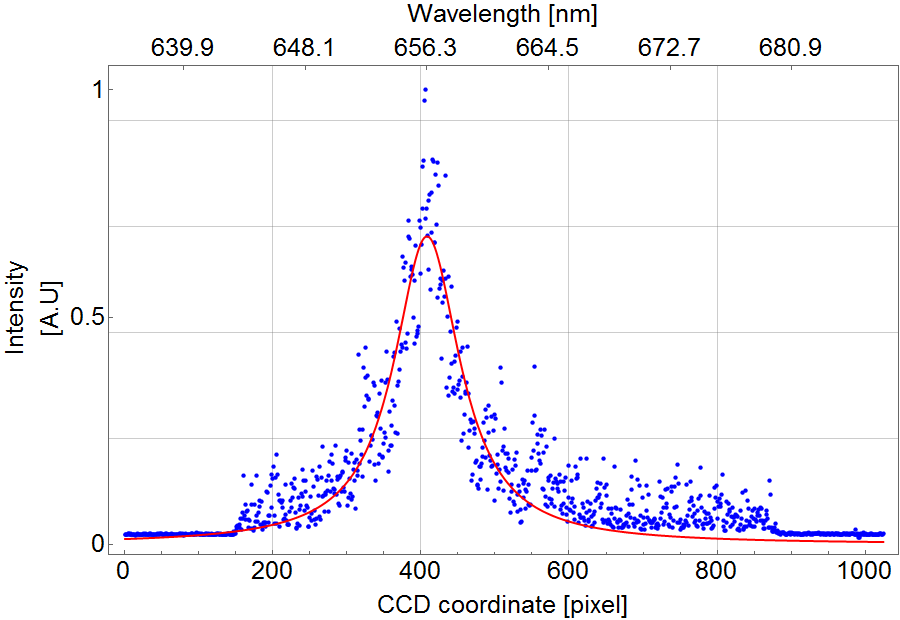
\includegraphics[width=0.8\textwidth]{figures/results/spectro/sample-lorentzian.png}
    %\end{figure}
    %Stark Broadening on the order of \SI{3}{\nm}.
%\end{frame}
%\begin{frame}{Spectroscopy measurements}{Radial density profile}
  %{\small Density minimum on the axis of the capillary.}
  %\begin{equation*}
    %\Delta N_e \sim \SI{0.4e18}{\per \cubic \cm}
  %\end{equation*}
  %{\small with}
  %\begin{equation*}
    %r_\text{ch}\approx \SI{50}{\um} \text{ and } N_e\left(0\right)\approx \SI{0.4e18}{\per\cubic\cm}.
  %\end{equation*}
  %\begin{figure}
    %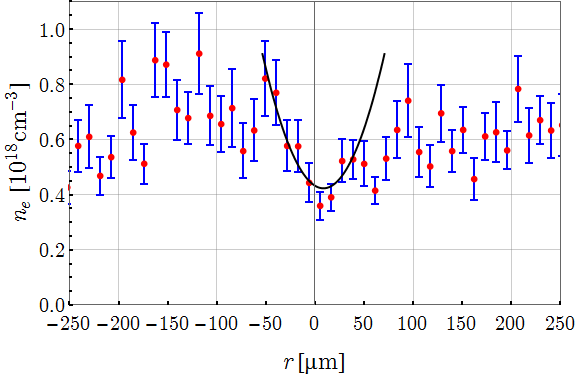
\includegraphics[height=120pt]{figures/results/spectro/parabolic_profile.png}
  %\end{figure}
%\end{frame}
%\begin{frame}{Longitudinal density profile}{System setup}
  %{\small Verify longitudinal homogeneity of the plasma density.}
  %\begin{figure}
    %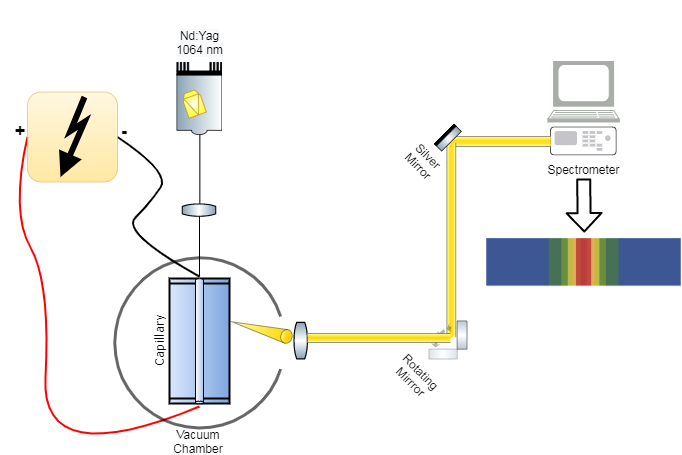
\includegraphics[height=130pt]{figures/results/spectro/longitudinal_system.png}
  %\end{figure}
  %The entire capillary length was imaged.
  %CCD camera \SI{1}{\us} gate--on time.
%\end{frame}
%\begin{frame}{Longitudinal density profile}{Result}
  %Mean plasma density $\bar{N}_e$ of
  %\begin{equation*}
      %\bar{N}_e \sim \SI{3e17}{\per\cubic\cm}.
  %\end{equation*}
  %\begin{figure}
    %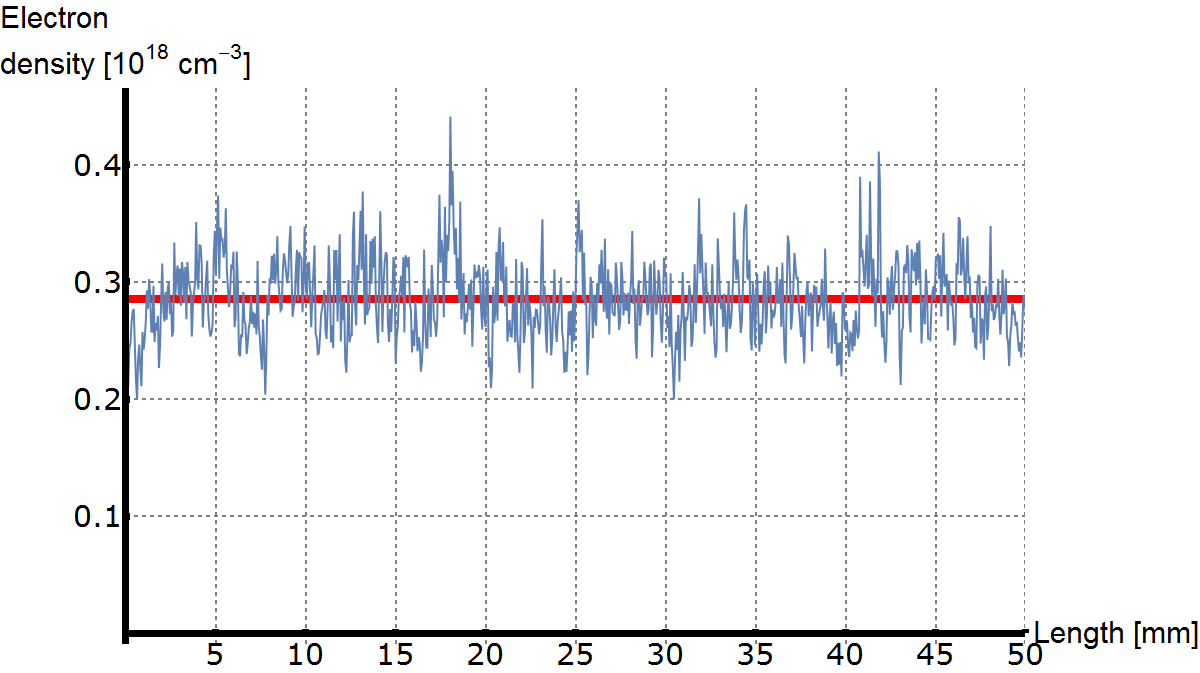
\includegraphics[height=110pt]{figures/results/spectro/longitudinal_profile.png}
  %\end{figure}

  %Plasma channel that can be used for guiding an intense laser pulse for LWFA accelerators.
%\end{frame}
%\subsection{Two stage capillary}
%\begin{frame}{Two stage capillary}
  %As said in the introduction, a "fish--bone" capillary may overcome the dephasing length limitation.
    %\begin{figure}
      %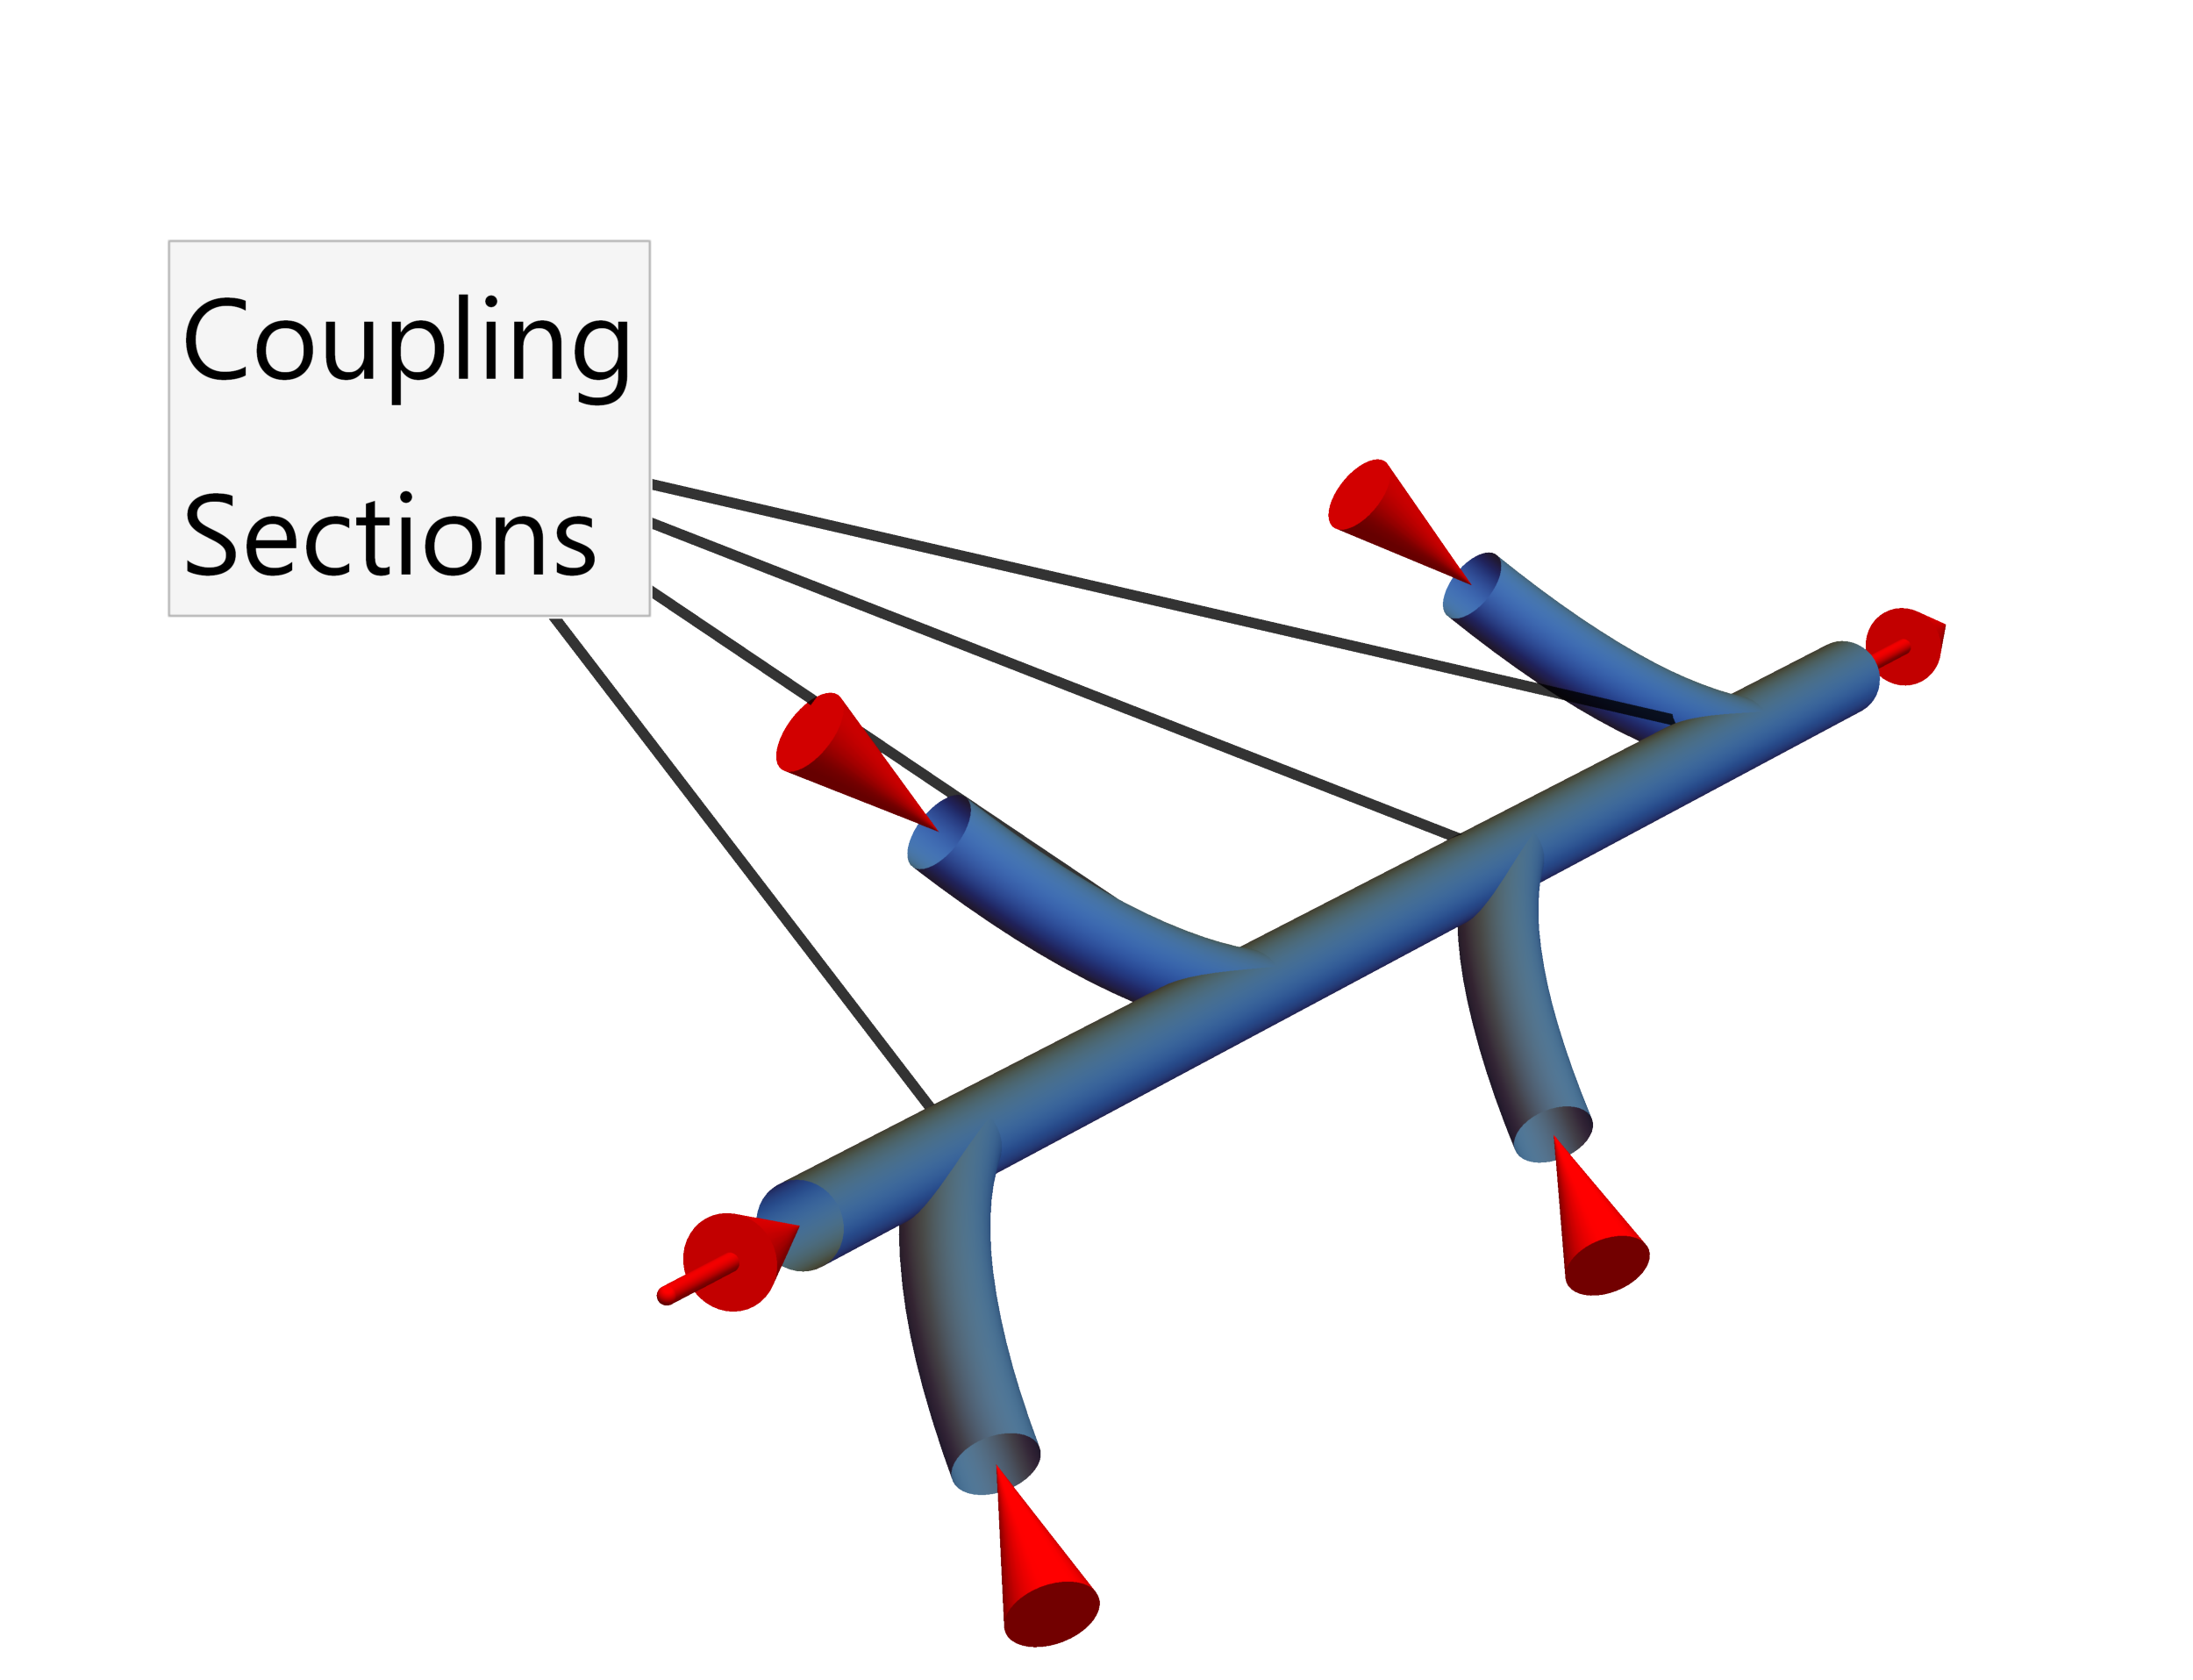
\includegraphics[width=0.2\textwidth]{figures/coupling_scheme.pdf}
    %\end{figure}
    %\begin{figure}
      %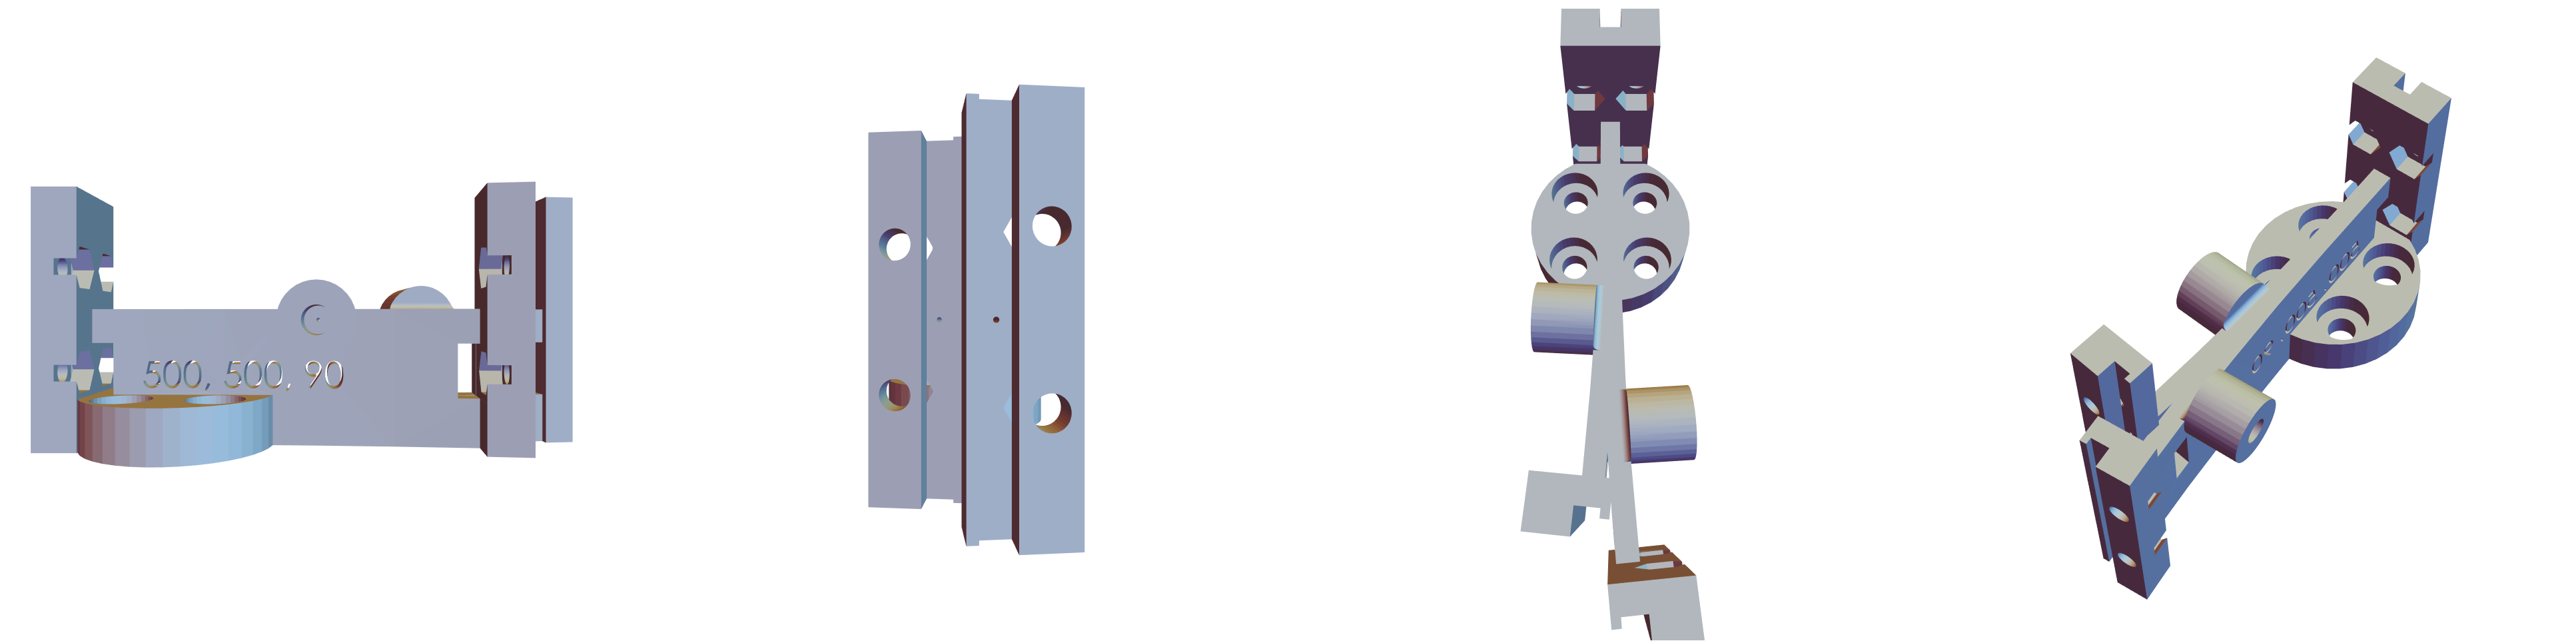
\includegraphics[width=0.8\textwidth]{figures/results/2stageCapillary/doublecapillary_cad.png}
    %\end{figure}
    %2 stage, Y--shape capillary.
%\end{frame}
\end{document}